\documentclass{report} 
\title{Strang}
\date{Started 5th June 2025}
\author{Malcolm}
\usepackage{amsmath} %import math
\usepackage{mathtools} %more math
\usepackage{amssymb} %for QED symbol
\usepackage{amsthm} %
\usepackage{bm}%bold math
\usepackage{graphicx} %import imaging
\graphicspath{{./images/}} %set imaging path
\begin{document}
\maketitle

\tableofcontents

\newpage

\chapter{Vectors and Matrices}
\section{Intuition for Dot product, Cosine formula, Schwarz and Triangle inequalities}
\textbf{Intuition for dot product}\\
The unit vectors $\bm{v}=(\cos\alpha,\sin\alpha)$ and $\bm{w}=(\cos\beta,\sin\beta)$ are plotted as follows
\begin{center}
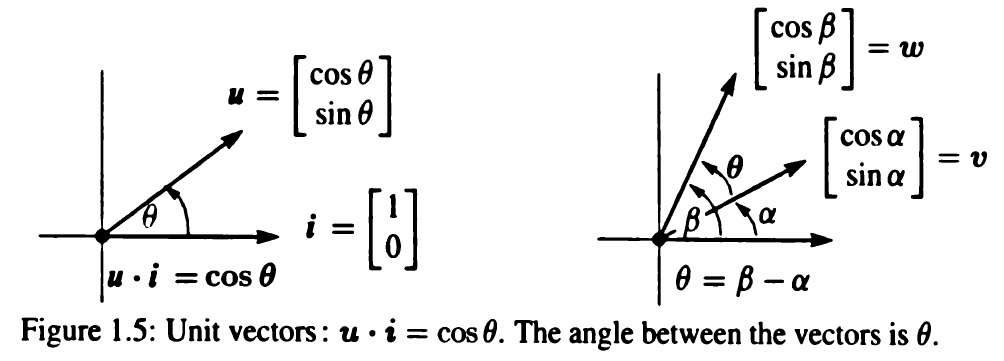
\includegraphics[width=10cm]{1}
\end{center}
See first that when fixed in this form, the magnitude of both vectors is 1, with an angle $\beta-\alpha$ between them. These unit vectors have dot product
\begin{equation*}
\bm{v}\cdot\bm{w}=\cos\alpha\cos\beta+\sin\alpha\sin\beta=\cos(\beta-\alpha)
\end{equation*}
We have $\theta$ as the angle between the two vectors; see that the sign of $\bm v\cdot\bm w$ tells us whether $\theta$ is below or above a right angle (due
to the cosine function being negative for its argument $>\pi/2$ and positive for $<\pi/2$):
\begin{center}
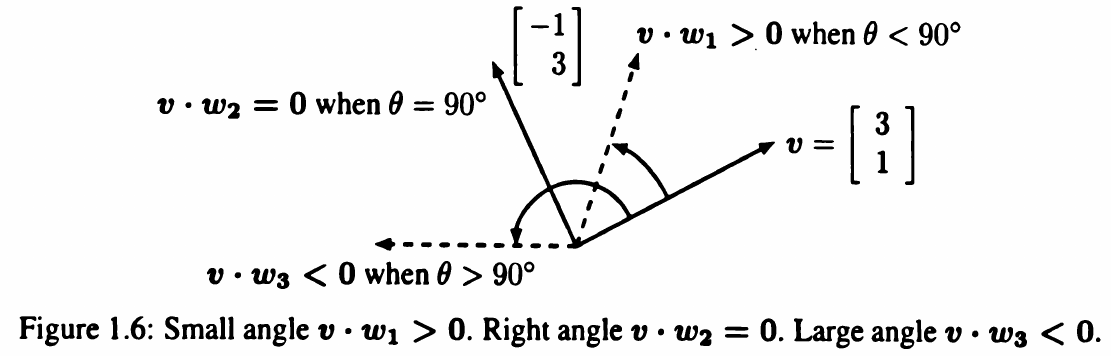
\includegraphics[width=9cm]{2}
\end{center}
(next page)\newpage
\noindent\textbf{Cont.}\\
The idea here is that the dot product reveals the exact angle $\theta$; for unit vectors $\bm u$ and $\bm U$, the dot product $\bm u\cdot\bm U$ is the cosine of 
$\theta$. Ths remains true in $n$ dimensions (not shown).\\
\vspace{1mm}\\
See that any $\bm{u}$ and $\bm{v}$ can be fixed in the above form by normalising their lengths to get
$\bm u=\bm v/||\bm v||$ and $\bm U=\bm w/||\bm w||$. After which their dot product would give $\cos\theta$. This leads us to the \textit{cosine formula}:
\begin{equation*}
\text{\textbf{Cosine formula}: }
\frac{\bm v\cdot\bm w}{||\bm v||\,||\bm w||}=\cos\theta\quad\text{ if $\bm v$ and $\bm w$ are nonzero vectors}
\end{equation*}
\textbf{Perpendicular vectors}\\
See that when the angle between $\bm v$ and $\bm w$ is $90^\circ$, its cosine is 0; this gives us a way to test this. Also see that for perpendicular vectors:
\begin{equation*}
||\bm v+\bm w||^2=||\bm v||^2+||\bm w||^2
\end{equation*}
because
\begin{equation*}
||\bm v+\bm w||^2=(\bm v+\bm w)\cdot(\bm v+\bm w)=\bm v\cdot\bm v+\bm v\cdot\bm w+\bm w\cdot\bm v+\bm w\cdot\bm w
\end{equation*}
where $\bm v\cdot \bm w=0$.\\
\vspace{1mm}\\
\textbf{Schwarz and Triangle inequalities}\\
First, see from the cosine formula that the dot product of $\bm v/||\bm v||$ and
$\bm w/||\bm w||$ never exceeds one (since $\cos\theta$ never exceeds one). This is the the 
\textit{Schwarz inequality}:
\begin{equation*}
\text{\textbf{Schwarz inequality}: }|\bm v\cdot\bm w|\leq||\bm v||\,||\bm w||
\end{equation*}
The \textit{Triangle inequality} comes directly from the Schwarz inequality:
\begin{equation*}
\text{\textbf{Triangle inequality}: }||\bm v+\bm w||\leq||\bm v||+||\bm w||
\end{equation*}
This can be seen from
\begin{equation*}
||\bm v+\bm w||^2=\bm v\cdot\bm v+\bm v\cdot\bm w+\bm w\cdot\bm v+\bm w\cdot\bm w
\leq||\bm v||^2+2||\bm v||\,||\bm w||+||\bm w||^2
\end{equation*}
The square root gives us the triangle equality (side 3 cannot exceed side 1 + side 2).
\newpage

\section{Intuition for column rank being equal to row rank}
If all columns are in the same direction, why does it happen that all the rows are the same direction?\\
\vspace{1mm}\\
Consider the matrix, see that column 2 is $m$ times column 1:
\begin{equation*}
\bm A=\left[\begin{array}{cc}
a&ma\\
b&mb
\end{array}\right]
\end{equation*}
See that the second row is just $b/a$ times the first row---if the column rank is 1, then the row rank is 1. See that transposing the matrix, we have
\begin{equation*}
\bm A=\left[\begin{array}{cc}
a(1)&b(1)\\
a(m)&b(m)
\end{array}\right]
\end{equation*}
which still has one independent column. Now consider the 3x3 case:
\begin{equation*}
\bm A=\left[\begin{array}{ccc}
a&ma&pa\\
b&mb&pb\\
c&mc&pc
\end{array}\right]
\end{equation*}
See that a similar deduction can also be made in this case, where the row rank of $A$ is equal to its column rank.\\
(next page)\newpage
\noindent\textbf{An informal proof}\\
Consider any matrix $\bm A$, suppose we go from left to right, looking for independent columns of $\bm A$ using the following procedure:
\begin{enumerate}
\item If column 1 of $\bm A$ is not zero, put it in matrix $\bm C$
\item If column 2 of $\bm A$ is not a multiple of column 1, put it in into $\bm C$
\item If column 3 of $\bm A$ is not a combination of columns 1 and 2, put it into $C$. \textit{continue}
\end{enumerate}
See that at the end $\bm C$ will have $r$ columns taken from $\bm A$, where $r$ is the rank of $\bm A$ and $\bm C$. While the $n$ columns of $\bm A$ are dependent, 
the $r$ columns of $\bm C$ will surely be independent.\\
\vspace{1mm}\\
For instance consider $\bm A$ with rank 2
\begin{equation*}
\bm A=\left[\begin{array}{ccc}
2&6&4\\
4&12&8\\
1&3&5
\end{array}\right]\quad\text{leads to}\quad \bm C=
\left[\begin{array}{cc}
2&4\\
4&8\\
1&5
\end{array}\right]
\end{equation*}
Now consider another matrix $\bm R$ to be multiplied by $\bm C$ such that 
$\bm A=\bm{CR}$. The first and third columns of $\bm A$ are already in $\bm C$, so those respective columns in $\bm R$ make up a \textit{identity matrix};
the second column of $\bm A$ is a multiple of the first, so we have
\begin{equation*}
\bm A=\bm{CR}\quad\text{is }\left[\begin{array}{ccc}
2&6&4\\
4&12&8\\
1&3&5
\end{array}\right]=
\left[\begin{array}{cc}
2&4\\
4&8\\
1&5
\end{array}\right]
\left[\begin{array}{ccc}
1&3&0\\
0&0&1
\end{array}\right]
\end{equation*}
(See that the $i$th row of $\bm A$ can be seen as a linear combination of the rows of $\bm R$ specified the $i$th row of $\bm C$. 
(or just consider $\bm A^T=\bm R^T\bm C^T$). We know that
\begin{enumerate}
\item $\bm C$ contains the full set of $r$ independent columns of $\bm A$.
\item $\bm R=[\bm{I\,\bm F}]$ contains the identity matrix $\bm I$ in the same $r$ columns that held $\bm C$.
\item The dependent columns of $\bm A$ are combinations of $\bm{CF}$ of the independent columns in $\bm C$.
\end{enumerate}
Where the matrix $\bm F$ goes into the other $n-r$ columns of $\bm R=[\bm{I\,\bm F}]$. ($\bm A=\bm{CR}$ becomes $\bm A=\bm{C[I,F]}=\bm{[C,CF]}=
[\text{indep cols of $\bm A$},\text{ dep cols of $\bm A$}]$ (in correct order).\\
\vspace{1mm}\\
See that $\bm C$ has the same column space as $\bm A$, and $\bm R$ \textit{has the same row space} as $\bm A$ (every row of $\bm A$ is a combination of the rows
of $\bm R$).\\
(next page)\newpage
\noindent\textbf{Cont.}\\
We had the example
\begin{equation*}
\bm A=\bm{CR}\quad\text{is }\left[\begin{array}{ccc}
2&6&4\\
4&12&8\\
1&3&5
\end{array}\right]=
\left[\begin{array}{cc}
2&4\\
4&8\\
1&5
\end{array}\right]
\left[\begin{array}{ccc}
1&3&0\\
0&0&1
\end{array}\right]
\end{equation*}
\textit{Here is an informal proof that the row rank of $\bm A$ equals the column rank of $\bm A$} (based from facts we already know)
\begin{enumerate}
\item The $r$ columns of $\bm C$ are independent (chosen that way from $\bm A$)
\item Every column of $\bm A$ is a combination of those $r$ columns of $\bm C$ (since $\bm A=\bm{CR}$)
\item The $r$ rows of $\bm R$ are independent (they contain the $r$ by $r$ matrix $\bm I$)
\item Every row of $\bm A$ is a combination of the $\bm r$ rows of $\bm R$
\end{enumerate}
See that for every column of $\bm A$ that goes into $\bm C$, a column of $\bm I$ goes into $\bm R$, where each column of $\bm I$ in $\bm R$ adds an independent row.\\
\vspace{1mm}\\
This means that the column rank of $\bm C$ (column space of $\bm A$) is always equal to the row rank of $\bm R$ (row space of $\bm A$)---the 
column rank of $\bm A$ is equal to the row rank of $\bm A$.\\
\vspace{1mm}\\
\textbf{More examples}\\
Rank 2:
\begin{equation*}
\left[\begin{array}{ccc}
1&2&3\\
4&5&6\\
7&8&9
\end{array}\right]=
\left[\begin{array}{cc}
1&2\\
4&5\\
7&8
\end{array}\right]
\left[\begin{array}{ccc}
1&0&-1\\
0&1&2
\end{array}\right]
\end{equation*}
Rank 2:
\begin{equation*}
\left[\begin{array}{cccc}
1&2&3&4\\
1&2&4&5
\end{array}\right]=
\left[\begin{array}{cc}
1&3\\
1&4
\end{array}\right]
\left[\begin{array}{cccc}
1&2&0&1\\
0&0&1&1
\end{array}\right]
\end{equation*}
Rank 1:
\begin{equation*}
\left[\begin{array}{cccc}
1&2&10&100\\
3&6&30&300\\
2&4&20&200
\end{array}\right]=
\left[\begin{array}{c}
1\\3\\2
\end{array}\right]
\left[\begin{array}{cccc}
1&2&10&100
\end{array}\right]
\end{equation*}
\newpage

\section{Ways to multiply $\bm{AB}=\bm C$}
\textbf{Multiplcation by columns of $\bm A$ and rows of $\bm B$}\\
A lesser known way to multiply $\bm{AB}$ is through considering the columns of $\bm A$ and the rows of $\bm B$ (contrary to the usual ideas where each 
entry of the result is a dot product of a row of $\bm A$ and column of $\bm B$):
\begin{center}
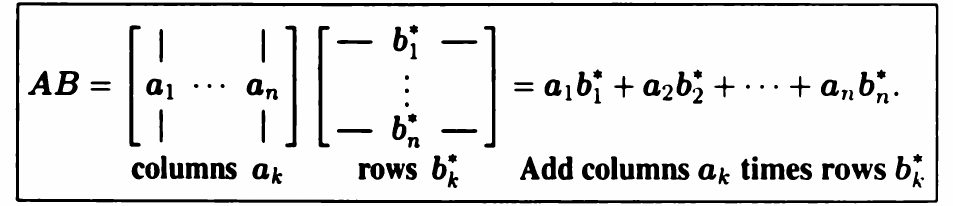
\includegraphics[width=10cm]{3}
\end{center}
We multiply each column of $\bm A$ by each row of $\bm B$; this gives us $n$ rank 1 matrices, which we then sum together; these matrices are called \textit{outer products}\\
\vspace{1mm}\\
(usually we see the $i$th column of the result as a linear combination of the columns of $\bm A$ specified by the $i$th column of $\bm B$. However
in this case the $i$th outer product is a matrix of the same size as the result, that contains all the contributions of the $i$th column of $\bm A$ to the final product.
By summing this over all $n$ columns of $\bm A$ we get the result.)\\
\vspace{1mm}\\
\textbf{Summary of methods}
\begin{center}
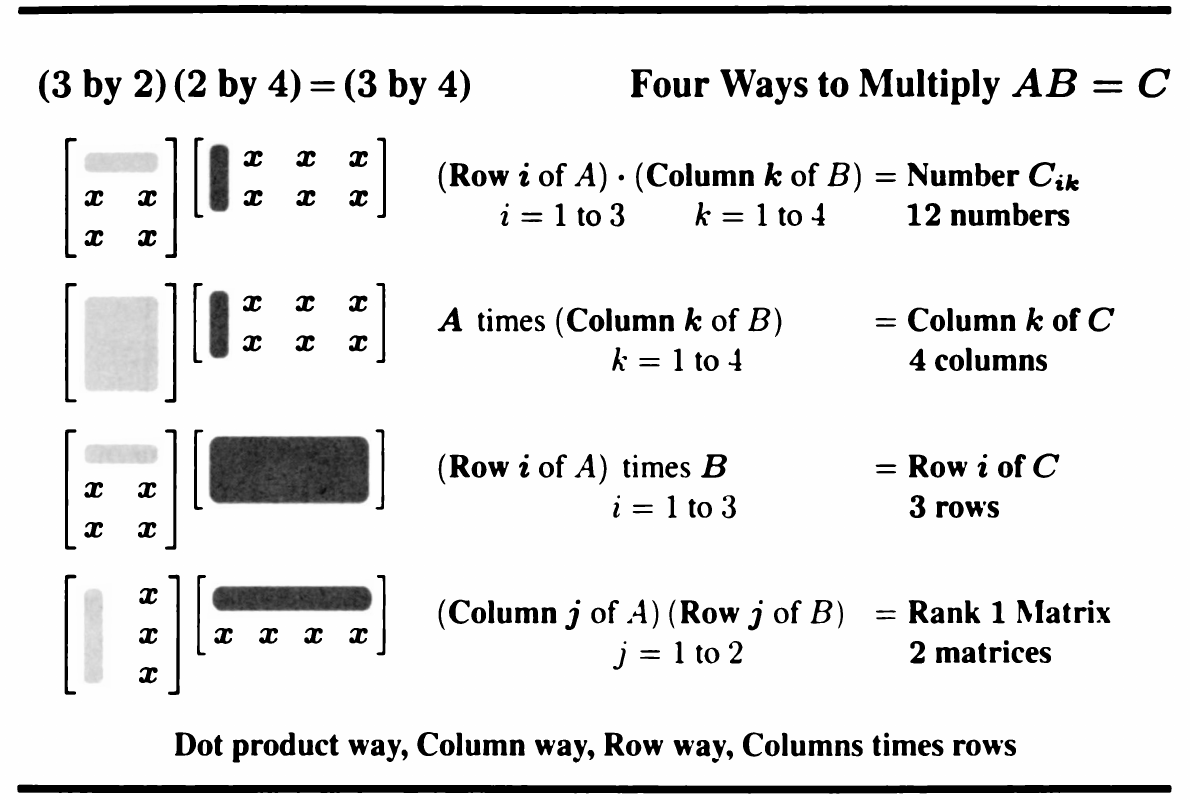
\includegraphics[width=10cm]{4}
\end{center}
(A nice way to intuit the the third method is to consider $(\bm{AB})^T=\bm B^T\bm A^T$; where the columns of $(\bm{AB})^T$ are the rows of $\bm{AB}$)
\newpage

\chapter{Solving linear equations $\bm{Ax}=\bm b$}\newpage

\section{Solutions to $\bm{Ax}=\bm b$}
Given a $n$x$n$ matrix $\bm A$ and an $n$x1 column vector $b$, there are three outcomes for the vector $\bm x$ that solves $\bm{Ax}=\bm b$.\\
\vspace{1mm}\\
First there may be \textit{no vector} $\bm x$ that solves $\bm{Ax}=\bm b$, or there may be exactly \textit{one} solution, or there may be \textit{infinitely many}
solution vectors $\bm x$. Here are the possibilities:\\
\vspace{1mm}\\
1. \textbf{Exactly one solution} to $\bm{Ax}=\bm b$ means that $\bm A$ has independent columns (only one particular linear combination of the columns of $\bm A$
leads to $\bm b$. That combination is specified by $\bm x$). $\bm A$ is full rank and the only solution to $\bm{Ax}=\bm{0}$ is $\bm x=\bm0$. 
$\bm A$ \textit{has an inverse matrix} $\bm A^{-1}$ (given $\bm b$, we can work backward to get $\bm x$ since only one $\bm x$ leads to $\bm b$).\\
\vspace{1mm}\\
2. \textbf{No solution} to $\bm{Ax}=\bm b$ means that $\bm b$ is not in the column space of $\bm A$, so $\bm A$ is not full rank.\\
\vspace{1mm}\\
3. \textbf{Infinitely many solutions}. See that when the columns of $\bm A$ are not independent (not full rank), then there are infinitely many ways to
produce the zero vector $\bm b=\bm0$ (this is the meaning of dependent columns), and so there are infinitely many solutions to $\bm{AX}=\bm0$.\\
\vspace{1mm}\\ 
Also see that if $\bm A$ is not full rank it means that its column space is some subspace, where
solutions only exist for $\bm b$ within that subspace.\\
\vspace{1mm}\\
As such, if there so happens to be a solution to $\bm{Ax}=\bm b$ then we can add any solution to $\bm{AX}=\bm0$:
\begin{equation*}
\bm A(\bm x+\alpha\bm X)=\bm A\bm x+\alpha\bm A\bm X=\bm b+\bm0=\bm b
\end{equation*}
For some constant $\alpha$, which gives us $\bm b$ again---we have infinitely many solutions.
\newpage

\section{Elimination and Back Substitution}
\textbf{Elimination}\\
We want to produce an \textit{upper triangular} matrix $\bm U$ from a square matrix $\bm A$. This is done through elimination; the procedure (for a 3x3 matrix) is as
follows (assuming no row exchanges):
\begin{enumerate}
\item Use the first equation(row) to produce zeros in column 1 below the first pivot.
\item Use the new second equation(row) to clear out column 2 below pivot 2 in row 2.
\item \textit{Continue to column 3}. The expected result is an upper triangular matrix $\bm U$.
\end{enumerate}
These steps can be carried out using elimination matrices $\bm E$.\\
\vspace{1mm}\\
Consider $\bm A$ and $\bm b$
\begin{equation*}
\bm A=\left[\begin{array}{ccc}
2&3&4\\
4&11&14\\
2&8&17
\end{array}\right]\quad
\bm b=\left[\begin{array}{c}
19\\55\\50
\end{array}\right]
\end{equation*}
$\bm E_{21}$ multiplies equation 1 by 2 and subtracts that from equation 2 to get a zero in the first column below the first pivot:
\begin{equation*}
\bm E_{21}=\left[\begin{array}{ccc}
1&0&0\\
-2&1&0\\
0&0&1
\end{array}\right]\implies
\bm E_{21}\bm A=\left[\begin{array}{ccc}
2&3&4\\
0&5&6\\
2&8&17
\end{array}\right],\quad
\bm E_{21}\bm b=\left[\begin{array}{c}
19\\17\\50
\end{array}\right]
\end{equation*}
(For intuition on the elimination matrices, consider the row perspective of matrix multiplication) This produced the desired zero in column 1. It changed equation 2.
To make the first pivot column zero, we subtract row 1 from row 3 using $\bm E_{31}$
\begin{equation*}
\bm E_{31}=\left[\begin{array}{ccc}
1&0&0\\
0&1&0\\
-1&0&1
\end{array}\right]\implies
\bm E_{31}\bm E_{21}\bm A=\left[\begin{array}{ccc}
2&3&4\\
0&5&6\\
0&5&13
\end{array}\right],\quad
\bm E_{31}\bm E_{21}\bm b=\left[\begin{array}{c}
19\\17\\31
\end{array}\right]
\end{equation*}
This completes elimination in column 1. Moving on to column 2 row 2 (the second pivot row). We use $\bm E_{32}$ to subtract equation 2 from equation 3
\begin{equation*}
\bm E_{31}=\left[\begin{array}{ccc}
1&0&0\\
0&1&0\\
0&-1&1
\end{array}\right]\implies
\bm U=\left[\begin{array}{ccc}
2&3&4\\
0&5&6\\
0&0&7
\end{array}\right],\quad
\bm c=\left[\begin{array}{c}
19\\17\\14
\end{array}\right]
\end{equation*}
$\bm E_{32}\bm E_{31}\bm E_{21}\bm A=\bm U$ is triangular. See that the same steps were applied to the right hand side 
$\bm b$ to produce a new right hand side $\bm c$.\\
(next page)\newpage
\noindent\textbf{Possible breakdown of elimination}\\
Elimination might fail. This occurs when zero appears in a pivot position---subtracting that zero from lower rows will not clear out the column
below that pivot. For example:
\begin{equation*}
\bm A=\left[\begin{array}{ccc}
2&3&4\\
4&6&14\\
2&8&17
\end{array}\right]\to
\left[\begin{array}{ccc}
2&3&4\\
0&0&6\\
0&5&13
\end{array}\right]=\bm B
\end{equation*}
A possible way to get around this would be to \textit{exchange} row 2 (with the zero pivot) for row (with the nonzero in that column), then carry out elimination
as per usual. This exchange is carried out using the permuation matrix $\bm P$:
\begin{equation*}
\bm{PB}=
\left[\begin{array}{ccc}
1&0&0\\
0&0&1\\
0&1&0
\end{array}\right]
\left[\begin{array}{ccc}
2&3&4\\
0&0&6\\
0&5&13
\end{array}\right]=
\left[\begin{array}{ccc}
2&3&4\\
0&5&13\\
0&0&6
\end{array}\right]
\end{equation*}
In this example the exchange produced $\bm U$ with nonzero pivots; normally there may be more columns eliminate before $\bm U$ is reached.\\
\vspace{1mm}\\
At times this exchange strategy may not work. This occurs when there is no pivot is available. Consider $\bm A'$:
\begin{equation*}
\bm A'=\left[\begin{array}{ccc}
2&3&4\\
4&6&14\\
2&3&17
\end{array}\right]\to
\left[\begin{array}{ccc}
2&3&4\\
0&0&6\\
0&0&13
\end{array}\right]=\bm U'
\end{equation*}
There is no second pivot in this case. This tells us that the matrix $\bm A'$ \textit{did not have full rank} (intuitively see that the non-pivot row can be expressed
as a linear combination of the other pivot rows, so the row space 
(which is equal to the row space of the original $\bm A'$ since the elimination steps are just linear combinations of the existing rows) 
is not full rank, and so the column space of the 
original $\bm A'$ is also not full rank.\\
\vspace{1mm}\\
In this case there will be nonzero solutions $\bm X$ to $\bm A'\bm X=0$. The columns of $\bm U'$ (and $\bm A'$) are not independent.\\
\vspace{1mm}\\
\textbf{Augmented matrix}\\
During elimination, in order to make sure that the operations on the matrix $\bm A$ are also executed on $\bm b$, one can 
\textit{include $\bm b$ as an extra column of $\bm A$}; this combination $[\bm A,\bm b]$ is called an \textit{augmented matrix}:
\begin{equation*}
\left[\begin{array}{cc}\bm A&\bm b\end{array}\right]=
\left[\begin{array}{cccc}
2&3&4&19\\
4&11&14&55\\
2&8&17&50
\end{array}\right]\xrightarrow{E}
\left[\begin{array}{cccc}
2&3&4&19\\
0&5&6&17\\
0&0&7&14
\end{array}\right]=
\left[\begin{array}{cc}\bm U&\bm c\end{array}\right]
\end{equation*}
(next page)\newpage
\noindent\textbf{Back Substitution to solve $\bm{Ux}=\bm c$}\\
Elimination (ideally) produces an upper triangular matrix $\bm U$ that has all zeros below the diagonal, with nonzero pivots. For instance we had, for some $\bm x$
\begin{equation*}
\bm{Ax}=\bm b,\quad\bm A=\left[\begin{array}{ccc}
2&3&4\\
4&11&14\\
2&8&17
\end{array}\right]\quad
\bm b=\left[\begin{array}{c}
19\\55\\50
\end{array}\right]
\end{equation*}
undergo elimination to to become
\begin{equation*}
\bm{Ux}=\bm c,\quad\bm U=\left[\begin{array}{ccc}
2&3&4\\
0&5&6\\
0&0&7
\end{array}\right]\quad
\bm c=\left[\begin{array}{c}
19\\17\\14
\end{array}\right]
\end{equation*}
See that this form allows us to easily solve the equations by going from bottom to top in a procedural manner, finding $x_3$, then $x_2$, then $x_1$:
\begin{enumerate}
\item\textit{Back substitution}: The last equation $7x_3=14$ gives $x_3=2$
\item\textit{Work upwards}: The next equation $5x_2+6(2)=17$ gives $x_2=1$
\item\textit{repeat}: The first equation $2x_1+3(1)+4(2)=19$ gives $x_1=4$
\end{enumerate}
giving us the only solution to this example $\bm x=(4,1,2)$. Remember the pivots need to be nonzero(full rank) for a single specific solution to be found.
\newpage

\section{Elimination matrices and inverse matrices}
\textbf{Elimination matrices}\\
The basic elimination step \textit{subtracts} a multiple $\ell_{ij}$ of equation $j$ from equation $i$. We always speak about \textit{subtractions} as elimination 
proceeds. For instance even if the first pivot $a_{11}=3$ and below it is
$a_{21}=-3$ where we could just add equation 1 to 2, we \textit{subtract} $\ell_{21}=-1$ \textit{times equation 1 from equation 2} (which gives
us the same result).\\
\vspace{1mm}\\
For instance here is the matrix that subtracts 2 times row 1 from row 3:
\begin{equation*}
\bm E_{31}=\left[\begin{array}{ccc}
1&0&0\\0&1&0\\-2&0&1\end{array}\right]
\end{equation*} 
If no row exchanges are needed, then three elimination matrices $\bm E_{21},
\bm E_{31},\bm E_{32}$ will produce three zeros below the diagonal to change $\bm A$ to the upper triangular $\bm U$(this just carries out elimination 
using matrices to represent each step).\\
\vspace{1mm}\\
\textbf{Inverse}\\
See that the \textit{inverse} of each matrix $\bm E_{ij}$ just \textit{adds back} $\ell_{ij}\,\cdot$ (row $j$) to row $i$. 
This leads to the inverse of their product $\bm E=\bm E_{32}\bm E_{31}\bm E_{21}$. We denote the inverse of $\bm E$ by $\bm L$. 
For instance, say some $\bm E$ subtracts 5 times row 1 from row 2, then $\bm E^{-1}$ adds 5 times row 1 to row 2:
\begin{equation*}
\bm E=\left[\begin{array}{ccc}
1&0&0\\-5&1&0\\0&0&1\end{array}\right],\quad
\bm E^{-1}=\left[\begin{array}{ccc}
1&0&0\\5&1&0\\0&0&1\end{array}\right]
\end{equation*}
(See that sequential application of these matrices, in either order, to some vector leads to no net change---as if we had multiplied by the identity.)\\
\vspace{1mm}\\
Now lets consider $\bm F$ which subtracts 4 times row 2 from row 3 (which might be a next step during elimination), naturally $\bm F^{-1}$ adds it back:
\begin{equation*}
\bm F=\left[\begin{array}{ccc}
1&0&0\\0&1&0\\0&-4&1\end{array}\right],\quad
\bm F^{-1}=\left[\begin{array}{ccc}
1&0&0\\0&1&0\\0&4&1\end{array}\right]
\end{equation*}
During elimination we would first apply $\bm E$ then $\bm F$, which is the same as applying $\bm{FE}$. Reversing the elimination would amount to 
$(\bm{FE})^{-1}$, which is the same as applying $\bm E^{-1}\bm F^{-1}$:
\begin{equation*}
\bm F\bm E=\left[\begin{array}{ccc}
1&0&0\\-5&1&0\\20&-4&1\end{array}\right]\quad\text{is inverted by}\quad
\bm E^{-1}\bm F^{-1}=\left[\begin{array}{ccc}
1&0&0\\5&1&0\\0&4&1\end{array}\right]
\end{equation*}
See that the product $\bm{FE}$ contains `20' but its inverse doesn't. In $\bm{FE}$, row 3 feels an effect of size 20 from row 1. However in $\bm E^{-1}\bm F^{-1}$ 
that doesn't happen.\\
(next page)\newpage
\noindent\textbf{$\bm L$ is the inverse of $\bm E$}\\
$\bm E$ is the product of all the elimination matrices $\bm E_{ij}$, it turns $\bm A$ into its upper triangular form $\bm{EA}=\bm U$ (assuming no row exchanges). 
The difficulty with $\bm E$ is multiplying all the separate elimination steps $\bm E_{ij}$ does not produce a good formula; illustrating 
$\bm E=\bm E_{32}\bm E_{31}\bm E_{21}$:
\begin{center}
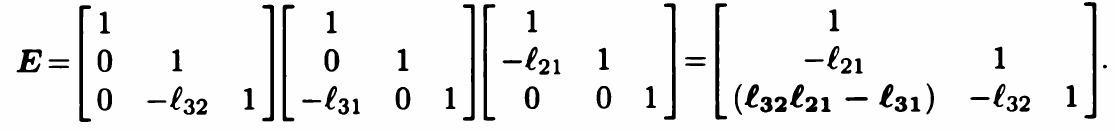
\includegraphics[width=10cm]{5}
\end{center}
See that the bottom left corner is dependent on multiple constants (since mutating the third row requries knowledge of the mutations that already occured to the
second row).\\
\vspace{1mm}\\
Now consider the inverse $\bm E^{-1}_{21}\bm E^{-1}_{31}\bm E^{-1}_{32}=\bm E^{-1}=\bm L$ (see that inverses need to be applied in reverse):
\begin{center}
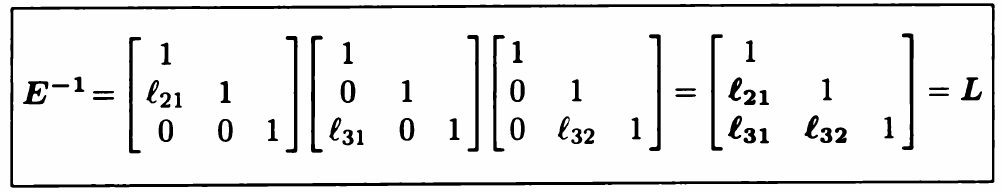
\includegraphics[width=10cm]{6}
\end{center}
(In the inverse matrix, the mutation of each row doesn't depend on previous mutations, so the multipliers fall into place in the lower triangular $\bm L$. 
Also see that the final matrix is only lower triangular because the elimination algorithm specifies that we don't manipulate the first row, and that we don't
manipulate the second row with the third row.)\\
\vspace{1mm}\\
This is why we might want to consider $\bm A=\bm{LU}$ to go back from triangular $\bm U$ to the original $\bm A$.
\newpage

\section{Gauss-Jordan elimination}
How would one compute the inverse of an $n$x$n$ matrix $\bm A$? Before answering that question, one might want to consider whether it is really necessary to know
$\bm A^{-1}$; although it is possible to find the solution to $\bm{Ax}=\bm b$ using $\bm x=\bm A^{-1}\bm{b}$, computing $\bm A^{-1}$ and taking $\bm A^{-1}\bm b$ is
a very slow way to find $\bm x$.\\
\vspace{1mm}\\
Say we want to compute $\bm A^{-1}$. This is equivalent to solving for $\bm{AX}=\bm I$. In that sense, by performing the manipulations on $\bm A$ to make it look
like $\bm I$. We essentially replicate the effect of $\bm A^{-1}$ on $\bm A$; by repeating those steps on the identity, 
it becomes as if we were taking $\bm A^{-1}\bm I=\bm A^{-1}$, allowing us to obtain the desired matrix.\\
\vspace{1mm}\\
This whole process can be done with an augmented matrix using \textit{Gauss-Jordan elimination}, where we essentially take steps to reduce $\bm A$ to reduced row
echelon form, while repeating said steps on the identity to obtain the inverse:
\begin{center}
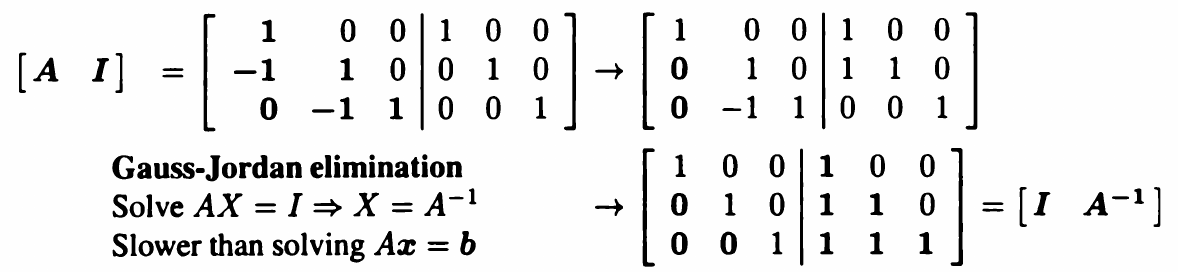
\includegraphics[width=10cm]{7}
\end{center}
The Gauss-Jordan essentially turns $[\bm A,\bm I]$ into $[I,\bm A^{-1}]$, where the elimination steps are essentially equivalent to multiplicaiton by $\bm A^{-1}$.
\newpage

\section{Proving $\bm A=\bm{LU}$}
Elimination is expressed by $\bm{EA}=\bm U$ and inverted by $\bm{LU}=\bm A$. It starts with $\bm A$ and ends with upper triangular $\bm U$, with each elimination step
being carried out by elimination matrices $\bm E_{ij}$. To invert one elimination step we add rows instead of subtracting:
\begin{center}
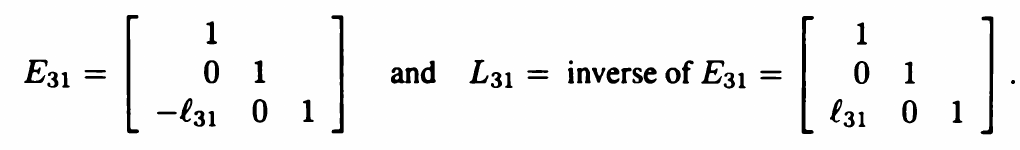
\includegraphics[width=10cm]{8}
\end{center}
Recall that $\bm E=\bm E_{32}\bm E_{31}\bm E_{21}$ gives us a fairly messy result:
\begin{center}
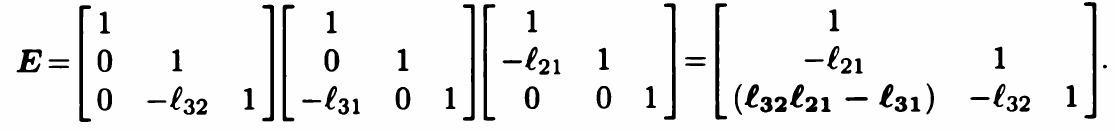
\includegraphics[width=10cm]{5}
\end{center}
while the inverse, $\bm E^{-1}=\bm E_{21}^{-1}\bm E_{31}^{-1}\bm E_{32}^{-1}=\bm L$ produces a much simpler result
\begin{center}
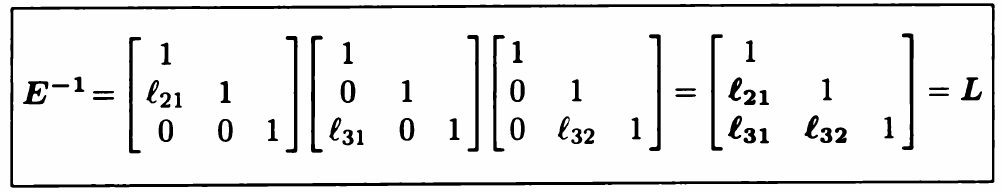
\includegraphics[width=10cm]{6}
\end{center}
We then have a elegant expression in $\bm A=\bm E^{-1}\bm U=\bm{LU}$. We now show that this equation holds over larger matrices of size $n$.\\
\vspace{1mm}\\
\textbf{Proof 1}\\
Following each step in elimination, consider the pivot rows that are subtracted from lower rows; see that these rows are not original rows of $\bm A$, since
they have been mutated by the previous elimination steps; they are instead rows of $\bm U$.\\
\vspace{1mm}\\
When computing the, say, third row of $\bm U$, we subtract multiples of earlier rows of $\bm U$:
\begin{equation*}
\text{Row 3 of $\bm U$}=(\text{Row 3 of $\bm A$})-\ell_{31}(\text{Row 1 of $\bm U$})-\ell_{32}(\text{Row 2 of $\bm U$})
\end{equation*}
Rewriting, see that
\begin{equation*}
\text{Row 3 of $\bm A$}=\ell_{31}(\text{Row 1 of $\bm U$})+\ell_{32}(\text{Row 2 of $\bm U$})+1(\text{Row 3 of $\bm U$})
\end{equation*}
Row $[\ell_{31},\ell_{32},1]$ is multiplying the matrix $\bm U$. This is \textit{exactly row 3 of $\bm A=\bm{LU}$}. All rows look like this regardless of the size of
$\bm A$. With no row exchanges, we have $\bm A=\bm{LU}$.\\
(next page)\newpage
\noindent\textbf{Proof 2}\\
Here is another proof. The idea here is to see elimination as removing one rank 1 matrix at a time---one column of $\bm L$ times one row of $\bm U$ from $\bm A$; 
where the problem becomes one size smaller with each iteration.\\
\vspace{1mm}\\
Elimination begins with pivot row = row 1 of $\bm A$. We multiply that pivot row by the numbers $\ell_{21}$, then $\ell_{31}$, and eventually $\ell_{n1}$; we subtract
the respective products from row 2, row 3, and eventually row $n$ of $\bm A$.
By choosing $\ell_{21}=a_{21}/a_{11}$, $\ell_{31}=a_{31}/a_{11}$ and so on until
$\ell_{n1}=a_{n1}/a_{11}$; now consider
if we also subtracted away the pivot row away from itself---this subtraction leaves zeros in column 1:
\begin{center}
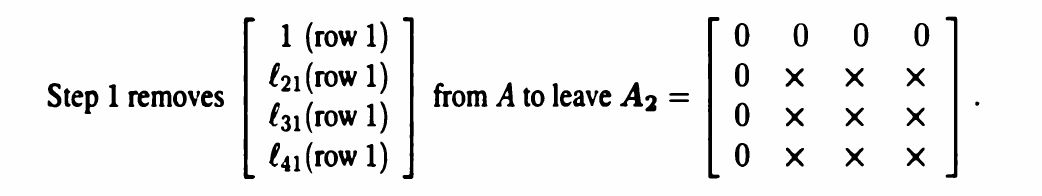
\includegraphics[width=10cm]{9}
\end{center}
The idea here is that we \textit{removed a rank 1 matrix} with columns made up of multiples of $\bm\ell_1=(1,\ell_{21},\ell_{31},\ell_{41},\ldots)$, 
scaled by
each respective entry of the first row of $\bm A$, which is also the first pivot row $\bm u_1$ of the final upper triangular matrix.\\
\vspace{1mm}\\
We continue with elimination in the second pivot column, using the second row as the pivot row; as before we also subtract the second pivot row from itself. 
See that this is again equivalent to subtracting a rank 1 matrix with basis
$\bm\ell_2=(0,1,\ell_{32},\ell_{42},\ldots)$. Recall that the second pivot row is the second row of the upper triangular matrix $\bm U$ in our factorisation.
\begin{center}
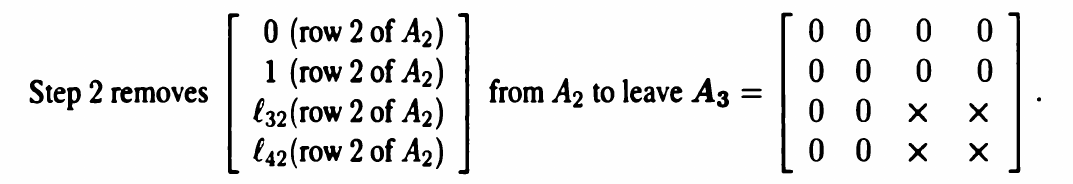
\includegraphics[width=10cm]{10}
\end{center}
Notice that both $\bm\ell_1$ and $\bm\ell_2$ are columns of $\bm L$.
We removed a column $\bm\ell_2$ times the second pivot row. Continuing in the same way, we successively remove columns with each step removing a column
$\bm\ell_j$ of $\bm L$ times a pivot row $\bm u_j$ of $\bm U$. See that this entire process can be depicted as
\begin{center}
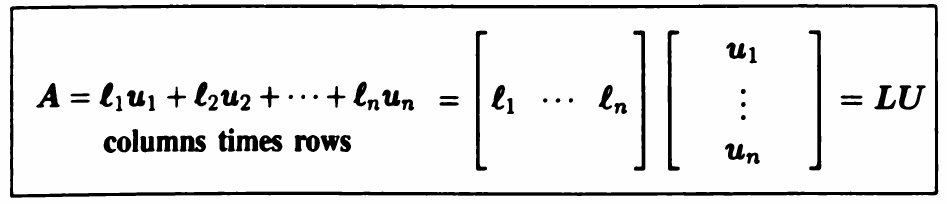
\includegraphics[width=10cm]{11}
\end{center}
Notice that $\bm U$ is upper triangular; the pivot row $u_k$ begins with $k-1$ zeros. $\bm L$ is lower triangular with 1's on the main diagonal. Column 
$\bm\ell_k$ also begins with $k-1$ zeros. (See that this proof makes use of the
idea that matrix multiplication can be seen as a sum of rank 1 matrices)
\newpage

\section{Permutation matrices}
\textbf{Examples}\\
Permutation matrices have a 1 in every row and a 1 in every column. All other entries are 0. When this matrix $\bm P$ multiplies a vector, it changes the order of 
its components; for instance:
\begin{center}
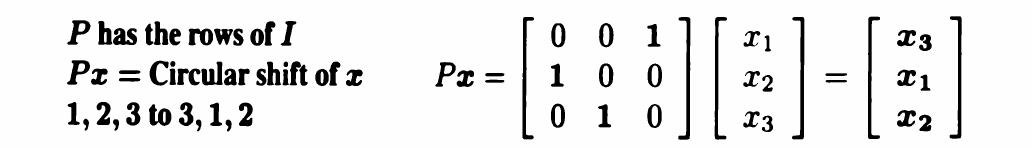
\includegraphics[width=10cm]{12}
\end{center}
(A nonzero $i$th entry on row $m$ of $\bm P$ means that row $i$ of $\bm x$ goes on that row $m$ in the result) Other examples include
\begin{center}
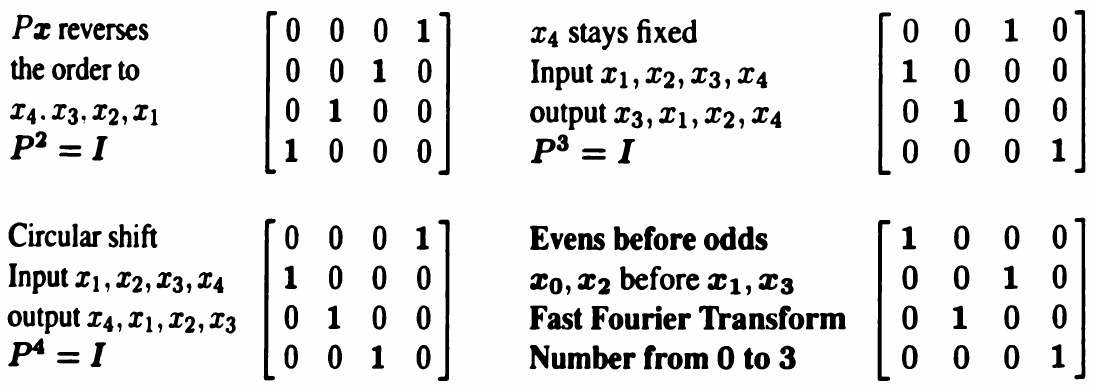
\includegraphics[width=10cm]{13}
\end{center}
Recall that elimination may require row exchanges. If $\bm A$ is invertible, then there is a permuation $\bm P$ to order its rows in advance, so that elimination
on $\bm{PA}$ meets no zeros in the pivot positions. Then $\bm{PA}=\bm{LU}$.\\
\vspace{1mm}\\
\textbf{Inverse}\\
We can intuit that the inverse of $\bm P$ is just its transpose:
\begin{center}
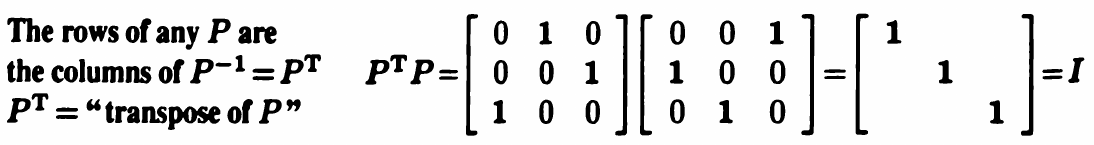
\includegraphics[width=10cm]{14}
\end{center}
(For instance, a nonzero entry in row 1 column 2 means `row 2 of $\bm x$ becomes row 1 of result'. Its transpose corresponds to a nonzero entry in 
row 2 column 1, so `row 1 of $\bm x$ becomes row 2 in the result'---reversing the change. This logic can be extrapolated to every other row.)\\
(next page)\newpage
\noindent\textbf{$\bm{PA}=\bm{LU}$ factorisation}\\
Recall that elimination may require row exchanges; consider for instance
\begin{center}
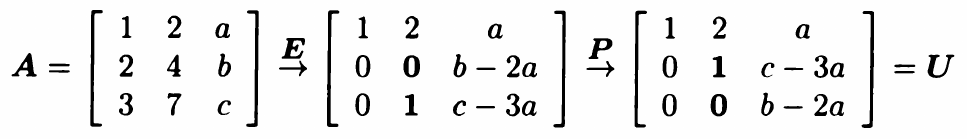
\includegraphics[width=12cm]{15}
\end{center}
To rescue elimination, $\bm P$ exchanced row 2 with 3, bringing 1 to the second pivot so elimination could continue.\\
\vspace{1mm}\\
See that we could order the rows in advance, first exchanging rows 2 and 3 to get $\bm{PA}$, then $\bm{LU}$ factorisation becomes $\bm{PA}=\bm{LU}$; the matrix
$\bm{PA}$ sails through elimination without seeing that zero pivot:
\begin{center}
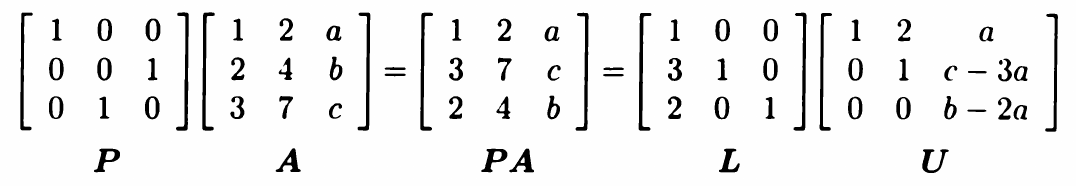
\includegraphics[width=12cm]{16}
\end{center}
We may require several row exchanges; in that case the an overall permutation $\bm P$ would include them all, still producing $\bm{PA}=\bm{LU}$. A useful way to keep
track of the permutations might be to add a column of indices at the end of $\bm A$ so that the original indices are displayed:
\begin{center}
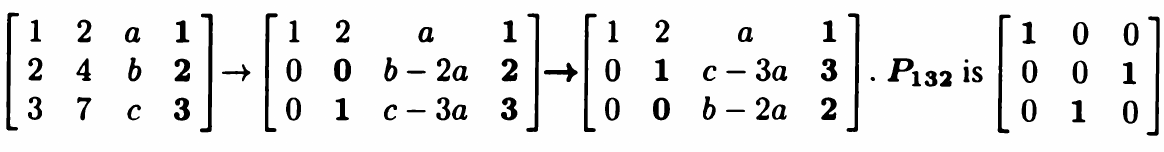
\includegraphics[width=12cm]{17}
\end{center}
\textbf{Column permutations}\\
We know that we can reorder rows using 
\begin{center}

\includegraphics[width=10cm]{18}
\end{center}
See that we can also reorder columns by applying a permutation matrix on the right:
\begin{center}
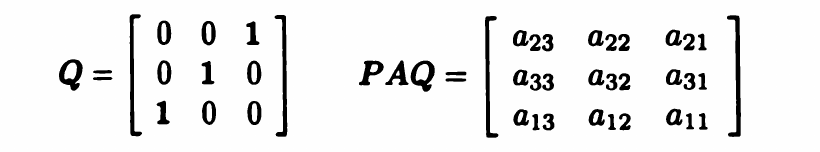
\includegraphics[width=8cm]{19}
\end{center}
Note that these two operations don't cover all possible permutations of the 9 entries in $\bm A$. The first index is constant on every row and the second index is
constant on every column.
\newpage

\section{Transposes and symmetric matrices}
\subsection{The transpose of $\bm{AB}$ is $\bm B^T\bm A^T$: Intuition}
We have
\begin{equation*}
(\bm{AB})^T=\bm B^T\bm A^T
\end{equation*}
Consider $\bm{AB}$. Computing the first \textit{row} of the result (the first column of $(\bm{AB})^T$); this can be seen as a linear combination of the 
\textit{rows} of $\bm B$ (the columns of $\bm B^T$) specified by the entries
in the first \textit{row} of $\bm A$ (the first column of $\bm A^T$).
\subsection{Showing $(\bm A^T)^{-1}=(\bm A^{-1})^T$}
Consider taking the transpose of $\bm A^{-1}\bm A$,
\begin{center}

\includegraphics[width=12cm]{20}
\end{center}
Similarly, transposing $\bm{AA}^{-1}=\bm I$ leads to $({\bm A}^{-1})^T\bm A^T=\bm I$. Notice especially that $\bm A^T$ \textit{is invertible exactly when $\bm A$ is 
invertible}.
\subsection{$\bm A^T\bm A$ is symmetric}
Choose any matrix $\bm A$, probably rectangular. Multiply $\bm A^T$ times $\bm A$, then the product $\bm S=\bm A^T\bm A$ is automatically a square symmetric matrix:
\begin{center}

\includegraphics[width=10cm]{21}
\end{center}
The matrix $\bm{AA}^T$ is also symmetric (see that their shapes permit multiplication in either order), note howerver that $\bm{AA}^T$ \textit{is a different matrix} 
from $\bm A^T\bm A$.
\newpage

\chapter{The Four Fundamental Subspaces}

\section{Reduced Row Echelon Form}
\textbf{Motivation}\\
Consider reducing a 2x4 matrix $\bm A$ to its reduced row echelon form $\bm R$:
\begin{center}
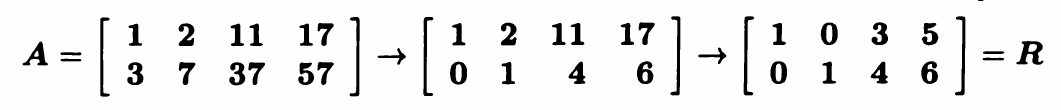
\includegraphics[width=12cm]{25}
\end{center}
See how the added upward elimination essentially inverted the a portion $\bm W$ of $\bm A$:
\begin{equation*}
\bm W=\left[\begin{array}{cc}1&2\\3&7\end{array}\right]
\end{equation*}
to turn that part of the matrix into the identity:
\begin{center}
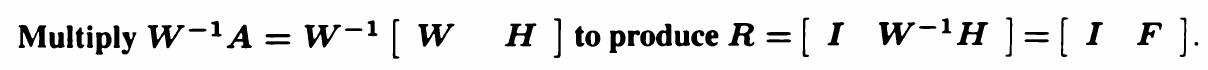
\includegraphics[width=12cm]{26}
\end{center}
We have $\bm H=\bm{WF}$, where $\bm H$ refers to the other parts of $\bm A$, and $\bm W$ the portion that was inverted---we can
combine the components of $\bm W$ (the first independent columns) to produce the other (dependent) columns. The matrix $\bm F$ specifies the parameters to do this:
\begin{center}
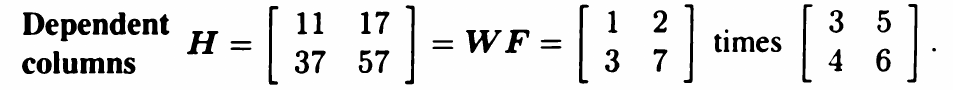
\includegraphics[width=10cm]{27}
\end{center}
See that the first $r$ independent columns of $\bm A$ locate the columns of $\bm R$ containing $\bm I$.
Also see that the last $m-r$ rows of $\bm R$ will be rows
of zeros (the dependent columns in the reduced form can be expressed in terms of the identity contained within that form, so there can't be any additional nonzero 
rows).\\
(next page)\newpage
\noindent\textbf{Algorithm}\\
Elimination goes a column at a time from left to right; after $k$ columns, that part of the matrix is in the reduced form, and we move to the $(k+1)$th column;
this new column has an upper part $\bm u$ and a lower part $\bm\ell$:
\begin{center}
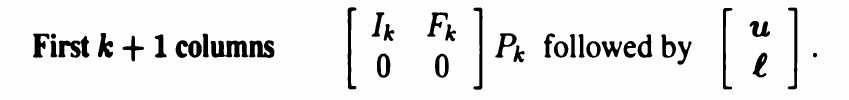
\includegraphics[width=10cm]{28}
\end{center}
The idea here is to decide whether this $(k+1)$th column joins $\bm I_k$ or $\bm F_k$.\\
\vspace{1mm}\\
See that if $\bm\ell$ is \textit{all zeros}, the new column is \textit{dependent} on the first $k$ columns; then $\bm u$ joins with $\bm F_k$ to produce 
$\bm F_{k+1}$.\\
\vspace{1mm}\\
If $\bm\ell$ is \textit{not} all zero, then the column is \textit{independent} of the first $k$ columns. Pick any nonzero in $\bm\ell$ as the pivot, move that row of 
$\bm A$ up into row $k+1$, then subtract multiples of that pivot row to zero out all the rest of column $k+1$ (eliminate up and down). If necessary, 
divide the row by its first nonzero entry to have a pivot of 1. Column $k+1$ joins $I_k$ (see that it adds a new nonzero row to the identity) to produce $I_{k+1}$.\\
\vspace{1mm}\\
Repeat for the next column and so on.\\
\vspace{1mm}\\
\textbf{Row operations}\\
There are three row operations allowed in elimination from $\bm A$ to $\bm R$:
\begin{enumerate}
\item Subtract a multiple of one row from another (below or above)
\item Divide a row by its first nonzero entry (to reach pivot 1)
\item Exchange rows (to move all zero rows to the bottom)
\end{enumerate}
A different series of steps could be used reach the same $\bm R$. But the result $\bm R$ can't change.
\newpage

\section{$\bm A=\bm{CR}$ factorisation}
We can apply elimination to reduce $\bm A$ to $\bm R_0$ (reduced echelon form with zero rows); then 
$\bm I$ in $\bm R_0$ locates the matrix $\bm C$ of \textit{independent columns} in $\bm A$. Removing any zero rows from $\bm R_0$ produces 
the row matrix $\bm R$ such that $\bm A=\bm{CR}$. For instance, 
\begin{center}
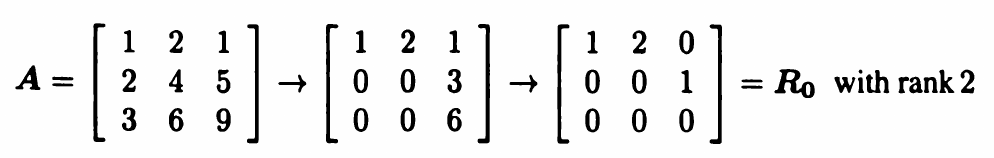
\includegraphics[width=10cm]{30}
\end{center}
where the independent columns of $\bm A$ are 1 and 3, and
\begin{equation*}
\bm R=\left[\begin{array}{ccc}
1&2&0\\0&0&1
\end{array}\right],\quad
\bm C=\left[\begin{array}{cc}
1&1\\2&5\\3&9
\end{array}\right]
\end{equation*}
so
\begin{center}
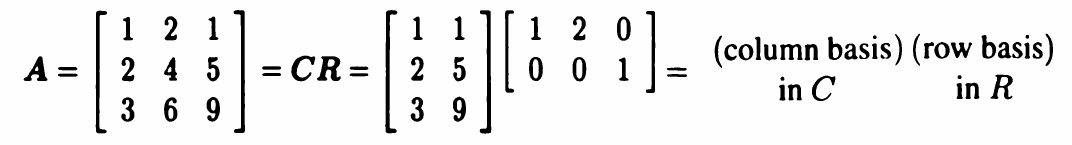
\includegraphics[width=12cm]{29}
\end{center}
\newpage

\section{Systematic nullspace computation}
Elimination gives us a systematic way to find a basis for the nullspace. Say we have
\begin{center}
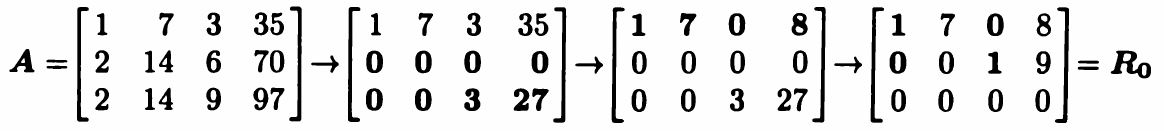
\includegraphics[width=12cm]{31}
\end{center}
Consider attempting to find a basis for the nullspace, meaning a basis for the solutions of $\bm{Ax}=\bm0$; say that $\bm{W^{-1}A}=\bm R_0$, then for some $\bm x$,
\begin{equation*}
\bm{Ax}=\bm0\implies\bm{W^{-1}Ax}=\bm{W^{-1}0}\implies\bm{R_0x}=\bm0
\end{equation*}
See that the elimination process doesn't change the space of solutions that satisfy $\bm{Ax}=\bm0$. Also see that using $\bm R$ instead of $\bm R_0$ only removes the 
redundant zero rows without removing any solutions.\\
\vspace{1mm}\\
Given some $\bm R$, we have a systematic way to find a basis for the nullspace: considering all the indices of $\bm x$ corresponding to dependent indices,
by letting one of those indices be 1 and the rest 0, we have a simple solution for $\bm{Rx}=\bm0$:
\begin{center}
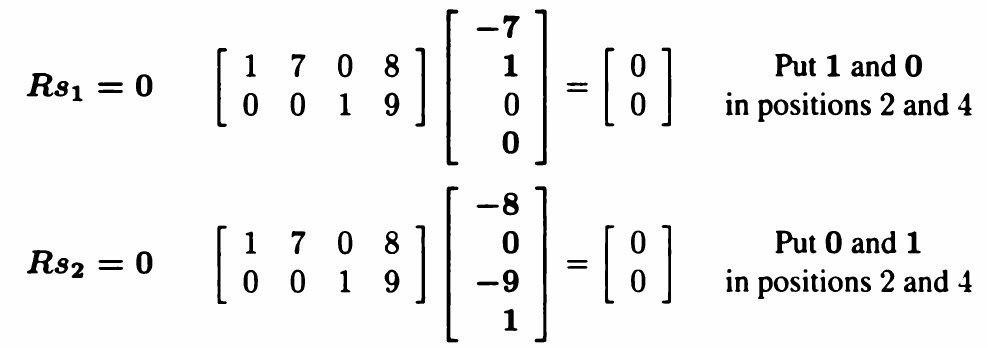
\includegraphics[width=10cm]{32}
\end{center}
See that if we were to write $\bm R$ as $[\bm I,\bm F]$, the solutions can be found in an algorithmic manner:
\begin{center}
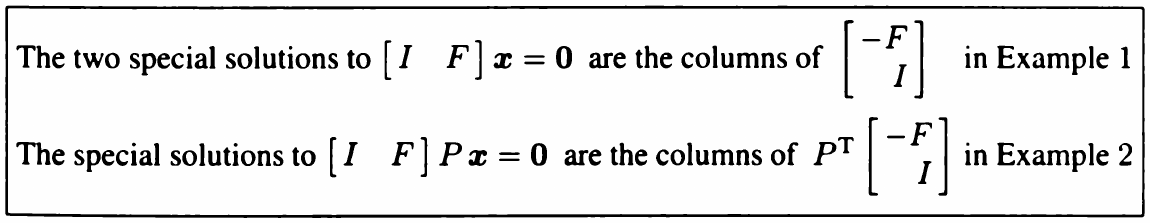
\includegraphics[width=12cm]{33}
\end{center}
The second case occurs should we have to permute $\bm R$ to reorder the independent columns. Recall that $\bm{PP}^T=\bm I$, and so
\begin{center}
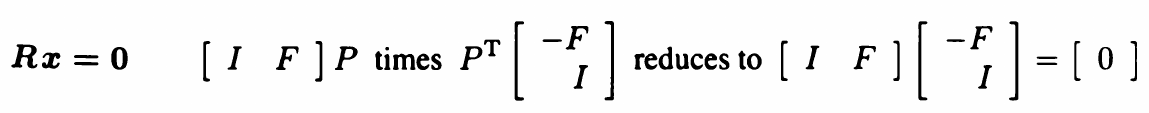
\includegraphics[width=12cm]{34}
\end{center}
(next page)\newpage
\noindent\textbf{Cont.}\\
To put these two ideas together, suppose the $m$x$n$ matrix $\bm A$ has rank $r$. To find the $n-r$ special solutions to $\bm{Ax}=\bm0$, compute the reduced row
echelon form $\bm R_0$ of $\bm A$; remove the $m-r$ zero rows of $\bm R_0$ to produce $\bm R=[\bm I,\bm F]\bm P$, where $\bm A=\bm{CR}$.\\
\vspace{1mm}\\
Then the special solutions to $\bm{Ax}=0$ are the $n-r$ columns of $\bm P^T\left[\begin{array}{c}-\bm F\\\bm I\end{array}\right]$.
\newpage

\section{The complete solution to $\bm{Ax}=\bm b$}
\textbf{Finding a particular solution}\\
We can reduce $\bm{Ax}=\bm b$ to a simpler system $\bm R_0\bm x=\bm d$ with the same solutions (if any). A useful aid here is to augment 
$\bm A$ with $\bm b$ to produce an augmented matrix $[\bm A,\bm b]$:
\begin{center}
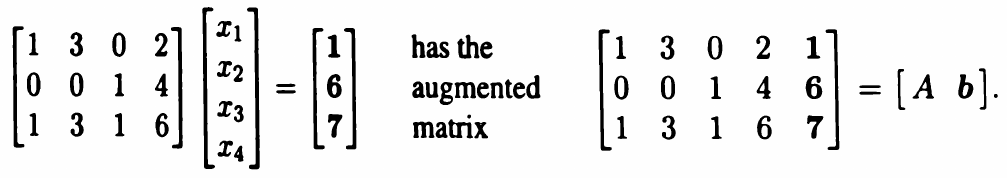
\includegraphics[width=11cm]{35}
\end{center}
Applying elimination to reach $\bm R_0$, the augmented part also undergoes the same elimination steps to produce a $\bm d$:
\begin{center}
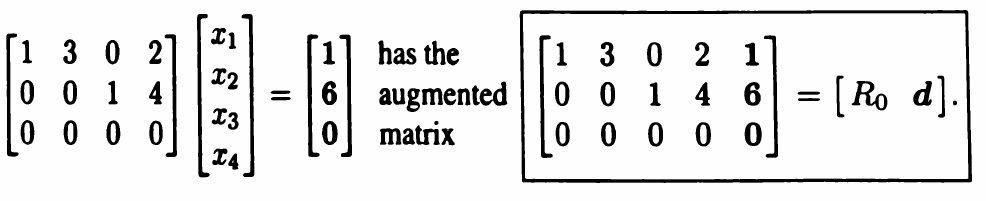
\includegraphics[width=11cm]{36}
\end{center}
For an easy solution $x_p$ we can \textit{choose the free variables to be 0}. In this case $x_2=x_4=0$, then the pivot variables can just be read off from $\bm d$:
\begin{center}
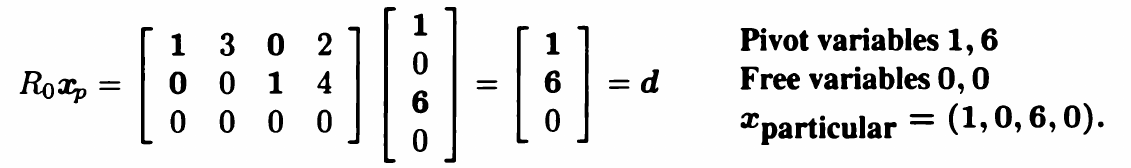
\includegraphics[width=12cm]{37}
\end{center}
See that for a solution to exist, the zero rows in $\bm R_0$ must also be zero in $\bm d$.\\
\vspace{1mm}\\
This procedure allows us to come up with a particular solution. For a complete solution, we consider any sum of the particular solution $x_p$ with any nullspace 
vectors $x_n$:
\begin{center}
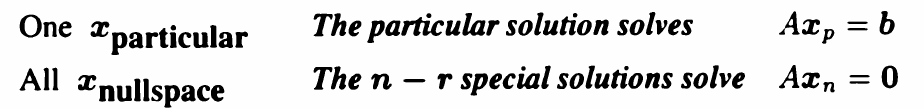
\includegraphics[width=10cm]{38}\\
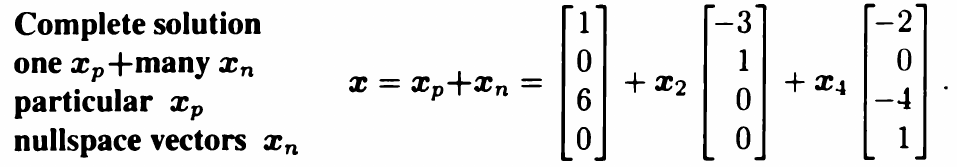
\includegraphics[width=11cm]{39}
\end{center}
The nullspace can be found as per outlined earlier (setting one variable to one and the rest to zero to get each nullspace basis vector). See 
that the complete solution includes all nullspace basis vectors, and 
that if the nullspace is just the zero vector then every particular solution $\bm x_p$ is the only solution to that $\bm b$.\\
(next page)\newpage
\subsection{Rank and solution}
\textbf{Full column rank}\\
In the case where $\bm A$ has \textit{full column rank}, every column has a pivot and the rank is $r=n$. The matrix is tall and thin ($m\geq n$). 
Row reduction puts $R=I$ at the top when $\bm A$ is reduced to $\bm R_0$ with rank $n$:
\begin{center}

\includegraphics[width=10cm]{40}\\
\end{center}
See that in this case the matrix has the following properties:
\begin{center}
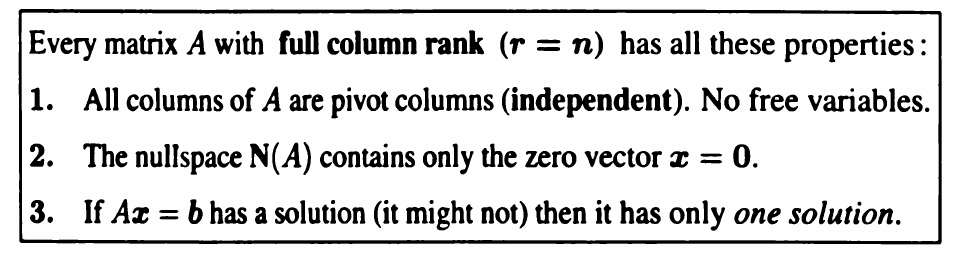
\includegraphics[width=11cm]{41}\\
\end{center}
With full column rank, $\bm{Ax}=\bm b$ will have \textit{one solution or no solution}. (think of a mapping from $n$ dimensional space into $m$ dimensional space
where $m\geq n$, there aren't enough vectors in $n$ space to encompass all of $m$ space, so there may be no solution for a particular vector in $m$ space; or see 
that the columns only span a $n$ dimensional hyperplane in a higher $m$ dimensional space---any $m$ dimensional vector not on that hyperplane has no solution)\\
\vspace{1mm}\\
\textbf{Full row rank}\\
The other case is full row rank---now $\bm{Ax}=\bm b$ has \textit{one or infinitely many solutions}. In this case $\bm A$ must be \textit{short and wide} ($m\leq n$);
the matrix has full row rank if $r=m$, where every row has a pivot.\\
\vspace{1mm}\\
(If $m<n$, then a nullspace consisting of more than just the zero vector exists and there will be multiple solutions to $\bm{Ax}=\bm b$.) See that a matrix like
this has the following properties:
\begin{center}
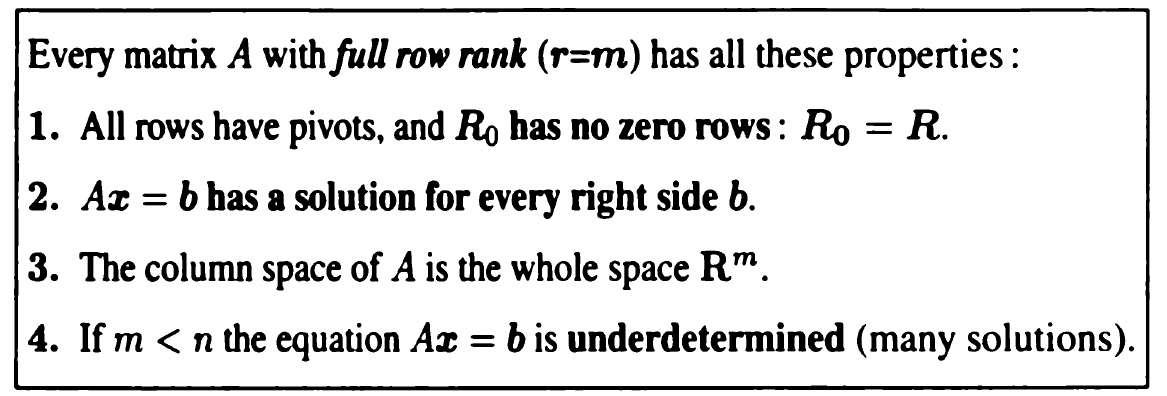
\includegraphics[width=10cm]{42}\\
\end{center}
(next page)\newpage
\noindent\textbf{Cont.}
\begin{center}
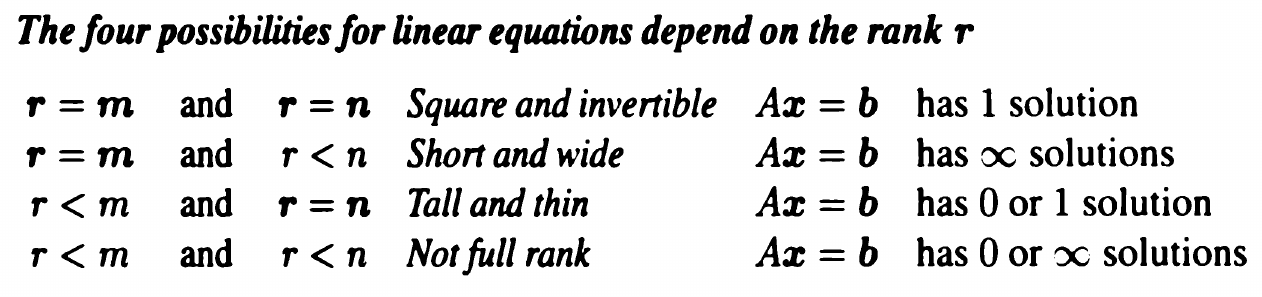
\includegraphics[width=12cm]{43}
\end{center}
If the matrix $\bm A$ is square and invertible, it indicates a mapping from $m=n=r$ space into that same space; the basis specified by $\bm A$ spans the whole of 
$r$ space
and there is only one linear combination of that basis that solves for $\bm{Ax}=\bm b$ (since $\bm A$ has linearly independent columns and therefore a trivial nullspace).\\
\vspace{1mm}\\
If the matrix is not full rank, then the columns span a hyperplane in the space equal to the row length, meaning some $\bm{Ax}=\bm b$ may not have a solution, and if
some $\bm b$ does lie within that hyperplane there will be infinite solutions to it (since the columns are not independent and therefore a nontrivial nullspace exists).\\
\vspace{1mm}\\
Their reduced row echelon form will fall into the following categories:
\begin{center}
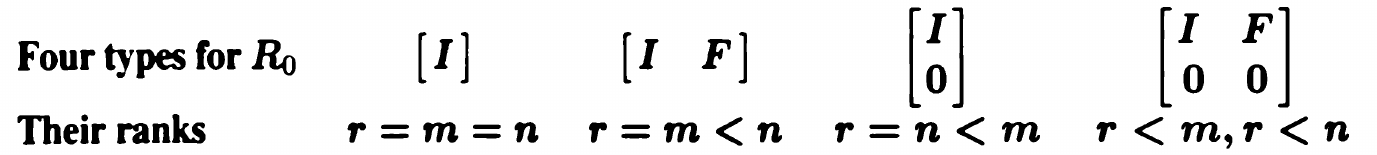
\includegraphics[width=12cm]{44}
\end{center}
Cases 1 and 2 have full row rank, case 3 has full column rank but not row rank, case 4 is not full rank.
See that in the last two cases, when $\bm{Ax}=\bm b$ is reduced to $\bm R_0\bm x=\bm d$, $\bm d$ must end in $m-r$ zeros for the equation to be solvable. $\bm F$ refers
to the top part of the dependent columns.
\newpage

\section{Intuition for four subspaces}
We have
\begin{center}
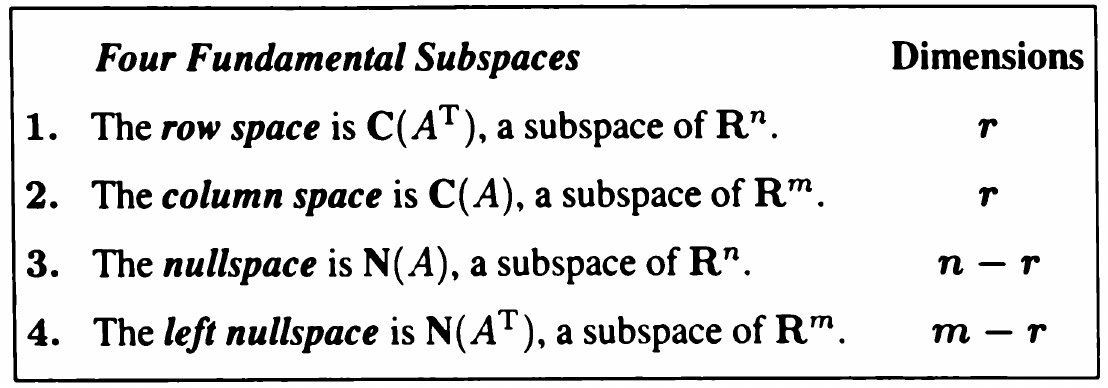
\includegraphics[width=10cm]{45}
\end{center}
\textbf{Column space of reduced form not the same as original matrix}\\
Note that although the reduced row echelon form provides the pivot positions to determine the row and column rank of a matrix, while the \textit{rows} of the rref form 
span the same row space as the original unreduced matrix, the columns of the rref form cannot act as substitutes for the original column space, instead only providing
information on dimensionality and on which original columns act as basis vectors for the column space. That is 
\begin{equation*}
\bm C(\bm A)\neq\bm C(\bm R_0)\quad\text{but}\quad\bm C(\bm A^T)=\bm C(\bm R_0^T)
\end{equation*}
(none of the row operations in elimination change the row space, but they do change the column space)\\
\vspace{1mm}\\
\textbf{Nullspace dimension is $n-r$}\\
The intuition for the dimension of $\bm N(A)$ being $n-r$ is clear from elimination, where each dependent column provides a new basis vector for the nullspace (we can
find a basis by substituting one free variable as 1 and the rest zero, repeating for all free variables), so the number of basis vectors equals the number of
dependent columns equals total columns minus independent columns---so $n-r$.
\vspace{1mm}\\
\textbf{Left nullspace dimensionality}\\
We know the dimensions for $\bm A$ is the same as that of $\bm A^T$. Transposing $\bm A$ gives us $m$ columns, of which we know $r$ are independent. So there are $m-r$ 
dependent columns which each provide a basis vector for the nullspace.
\newpage

\section{$\bm A=\bm{CR}$ and Block elimination}
The earlier notes on the rref form introduced it as a simple way to express the entire matrix in terms of its dependent rows, where for a matrix $\bm A$, with independent
components $\bm W$ and dependent components $\bm H$, reduction to rref looks like:
\begin{equation*}
\bm A=\left[\begin{array}{cc}W&H\end{array}\right]\implies
\bm W^{-1}\bm A=\bm W^{-1}\left[\begin{array}{cc}W&H\end{array}\right]=
\left[\begin{array}{cc}I&W^{-1}H\end{array}\right]
\end{equation*}
See that we can recover the dependent components of $\bm H$ with $\bm W^{-1}\bm H$ by multiplying it by the independent columns $\bm W$, so
\begin{equation*}
\bm A=\underbrace{\bm W}_{\bm C}\underbrace{\left[\begin{array}{cc}I&W^{-1}H\end{array}\right]}_{\bm R}
\end{equation*}
where $\bm C$ means the same thing as $\bm W$, that is, the independent columns of $\bm A$. See that
$\bm W$ is gauranteed to be square since row and column rank are equal.\\
\vspace{1mm}\\
\textbf{Block elimination}\\
The above doesn't show how the zero rows in $\bm R_0$ (if they exist) are redundant. 
We can develop a better idea of elimination if we consider working with blocks of the original $\bm A$. This is called block elimination; consider reducing
a matrix $\bm A$ with rank $r$ to rref using the following three steps:\\
\vspace{1mm}\\
\textbf{Step 1}: Exchange columns of $\bm A$ using $\bm P_C$ and exchange rows of $\bm A$ using $\bm P_R$ to put the $r$ independent columns first and $r$ independent rows 
first. This looks like
\begin{equation*}
\bm P_R\bm A\bm P_C=\left[\begin{array}{cc}
\bm W&\bm H\\
\bm J&\bm K\end{array}\right]
\end{equation*}
$\left[\begin{array}{c}\bm W\\\bm J\end{array}\right]$ has full column rank and 
$\left[\begin{array}{cc}\bm W&\bm H\end{array}\right]$ has full row rank. See that $\bm W$ is a square matrix with full rank $r$ and is therefore invertible.\\
\vspace{1mm}\\
\textbf{Step 2}: Multiply the top rows by $\bm W^{-1}$:
\begin{equation*}
\left[\begin{array}{cc}
\bm W&\bm H\\
\bm J&\bm K\end{array}\right]\to
\left[\begin{array}{cc}
\bm I&\bm W^{-1}\bm H\\
\bm J&\bm K\end{array}\right]
\end{equation*}
\textbf{Step 3}: Subtract $\bm J[\begin{array}{cc}\bm I&\bm W^{-1}\bm H\end{array}]$
from the $m-r$ rows $[\begin{array}{cc}\bm J&\bm K\end{array}]$ to produce
$[\begin{array}{cc}\bm0&\bm0\end{array}]$:
\begin{equation*}
\left[\begin{array}{cc}
\bm I&\bm W^{-1}\bm H\\
\bm J&\bm K\end{array}\right]\to
\left[\begin{array}{cc}
\bm I&\bm W^{-1}\bm H\\
\bm 0&\bm 0\end{array}\right]
\end{equation*}
To understand why $\bm J\bm W^{-1}\bm H=\bm K$, we know that the first $r$ rows 
$[\begin{array}{cc}\bm I&\bm W^{-1}\bm H\end{array}]$ are linearly independent, and since $\bm A$ has rank $r$, the lower rows $[\begin{array}{cc}\bm J&\bm K\end{array}]$ 
must be combinations of the upper rows. These combinations must be given by $\bm J$ to get
the first $r$ columns correct: $\bm{JI}=\bm J$. Then $\bm J$ times $\bm W^{-1}\bm H$ must equal $\bm K$ to make the last columns correct.\\
(next page)\newpage
\noindent\textbf{Cont.}\\
We have block elimination as the following transformations:
\begin{center}
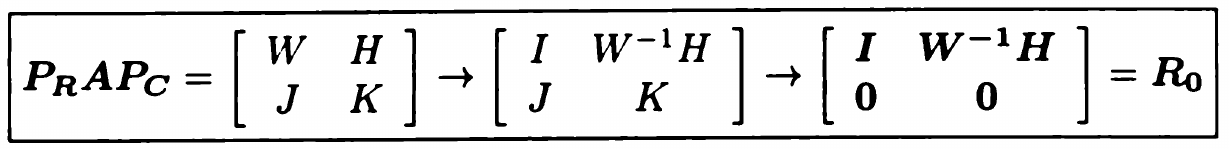
\includegraphics[width=12cm]{47}
\end{center}
We can, in a manner similar to the steps taken, factor out parts of $\bm A$ as follows to acquire the reduced row echelon form; for step 2:
\begin{equation*}
\bm P_R\bm A\bm P_C=\left[\begin{array}{cc}
\bm W&\bm H\\
\bm J&\bm K\end{array}\right]=
\left[\begin{array}{cc}
\bm W&\bm 0\\
\bm 0&\bm 1\end{array}\right]
\left[\begin{array}{cc}
\bm I&\bm W^{-1}\bm H\\
\bm J&\bm K\end{array}\right]
\end{equation*}
For step 3:
\begin{equation*}
\left[\begin{array}{cc}
\bm W&\bm 0\\
\bm 0&\bm 1\end{array}\right]
\left[\begin{array}{cc}
\bm I&\bm W^{-1}\bm H\\
\bm J&\bm K\end{array}\right]=
\left[\begin{array}{cc}
\bm W&\bm 0\\
\bm 0&\bm 1\end{array}\right]
\left[\begin{array}{cc}
\bm 1&\bm 0\\
\bm J&\bm 0\end{array}\right]
\left[\begin{array}{cc}
\bm I&\bm W^{-1}\bm H\\
\bm 0&\bm 0\end{array}\right]
\end{equation*}
The result is
\begin{equation*}
\bm P_R\bm A\bm P_C=
\left[\begin{array}{cc}
\bm W&\bm 0\\
\bm J&\bm 0\end{array}\right]
\left[\begin{array}{cc}
\bm I&\bm W^{-1}\bm H\\
\bm 0&\bm 0\end{array}\right]=\left[\begin{array}{c}
\bm W\\
\bm J\end{array}\right]
\left[\begin{array}{cc}
\bm I&\bm W^{-1}\bm H\end{array}\right]
\end{equation*}
See that this is just the $\bm A=\bm{CR}$ factorisation, but this time showing that the zero rows are redundant rather than just using a reduced form where zero rows don't
exist. Another way of writing this result is
\begin{center}
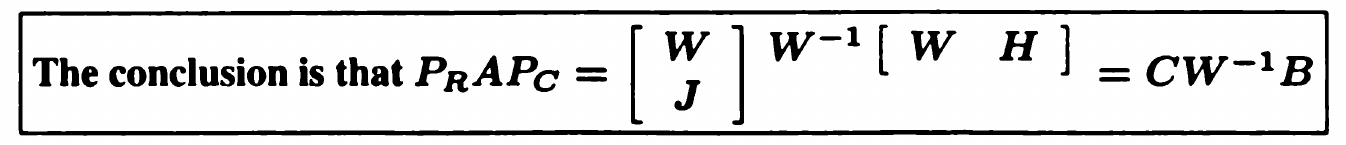
\includegraphics[width=12cm]{48}
\end{center}
\newpage

\chapter{Orthogonality}

\section{Orthogonal subspaces}
Recall that two vectors $\bm v$ and $\bm w$ are orthogonal if $\bm v^T\bm w=0$. To say that two subspaces are orthogonal means that every vector in one space
is orthogonal to every vector in the other space.\\
\vspace{1mm}\\
We can make the claim that for any matrix $\bm A$, \textit{the nullspace of $\bm A$ is orthogonal to the row space of $\bm A$.} To see this just consider $\bm{Ax}=\bm0$:
\begin{center}
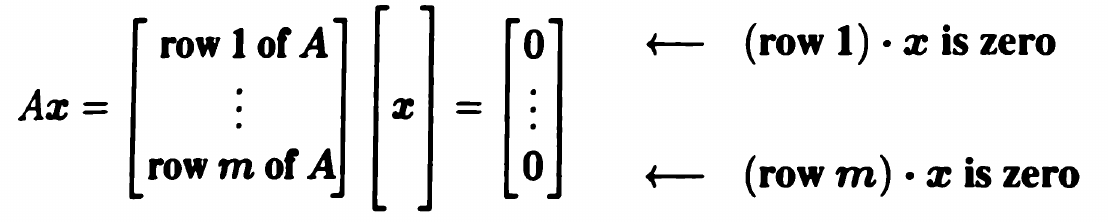
\includegraphics[width=10cm]{49}
\end{center}
Every row has a zero dot product with $\bm x$. Then every combination of the rows is perpendicular to $\bm x$. That is, the whole row space $\bm C(\bm A^T)$ is orthogonal to 
the nullspace $\bm N(\bm A)$ in $n$ dimensional space (since $\bm A^T$ has $n$ rows). Another way to show this is
\begin{center}

\includegraphics[width=10cm]{50}
\end{center}
See that we can analagously reason that the \textit{the column space $\bm C(\bm A)$ and the left nullspace $\bm N(\bm A^T)$ are perpendicular inside $m$ dimensional space}.\\
(next page)\newpage
\noindent\textbf{Cont.}\\
See that the only common vector between two orthogonal subspaces would be the zero vector (we can't sum the columns of a matrix to produce a vector orthogonal
to all the columns). There is a very important restriction on the dimension of any
two orthogonal subspaces:
\begin{center}

\includegraphics[width=10cm]{51}
\end{center}
For instance, the row space of a matrix is a subspace of dimension $r$ in $n$ space, and its orthogonal complement, by construction, will have dimensionality $n-r$.
\subsection{Orthogonal complements}
When two orthogonal subspaces account for the whole space, they are called \textit{orthogonal complements}. The orthogonal complement of $\bm V$ is written as $\bm V^\perp$.
The row space and the nullspace, as well as the column space and left nullspace, are
instances of orthogonal complements:
\begin{center}

\includegraphics[width=10cm]{52}
\end{center}
\subsection{Intuition for $\bm x=\bm x_\text{row}+\bm x_\text{null}$}
See that because the row space and the nullspace combined span the entire $n$ space, we can say that any vector in $\mathbb{R}^n$ can be expressed as a sum of vectors from 
both subspaces. That is, any vector $\bm x$ in $\mathbb{R}^n$ is the sum $\bm x=\bm x_\text{row}+\bm x_\text{null}$ of its row space component and its nullspace component.
Any vector $\bm y$ in $\mathbb{R}^m$ is the sum $\bm y=\bm y_\text{col}+\bm y_\text{null}$ of its column space component and its left nullspace component from 
$\bm N(\bm A^T)$:
\begin{center}
\includegraphics[width=9.8cm]{53}
\end{center}
(next page)\newpage
\subsection{$\bm A$ is invertible from the row space to the column space}
Consider again the illustration from the previous page:
\begin{center}
\includegraphics[width=12cm]{53}
\end{center}
Every vector in $\bm{Ax}$ is in the column space; that is obvious. Every $\bm x$ comes from $\mathbb{R}^n$ space, which is made up of the the row space $\bm C(\bm A^T)$ and
its orthogonal complement, the nullspace $\bm N(\bm A)$. In that context, every candidate $\bm x$ either comes from the nullspace, which would map to $\bm0$, or
the row space, which would then map to some $\bm b$ in the column space---every $\bm b$ in the column space can be found by some $\bm{Ax}$ with $\bm x$ from the 
row space.\\
\vspace{1mm}\\
We can also go on to say that \textit{every vector $\bm b$ in the column space comes from exactly one vector $\bm x_r$ in the row space}. Proof: If $\bm{Ax}_r=\bm{Ax}_{r}'$,
the difference $\bm{x}_r-\bm{x}_{r}'$ is in the nullspace (since 
$\bm A(\bm{x}_r-\bm{x}_{r}')=\bm 0$); however, should $\bm{x}_r$ and $\bm{x}_{r}'$ come from the row space, then $\bm{x}_r-\bm{x}_{r}'$ would also have to be in the row
space. The only way for a vector to be in both the nullspace and the row space would be if it were the zero vector; so $\bm{x}_r-\bm{x}_{r}'=\bm 0$ and 
$\bm{x}_r=\bm{x}_{r}'$.\\
\vspace{1mm}\\
So $\bm A$ maps every row space component to a specific column space component; see that there is an $r$ by $r$ invertible matrix hiding inside $\bm A$ if we throw away the 
two nullspaces. $\bm A$ \textit{is invertible from the row space to the column space}.
\newpage

\section{$\bm A^T\bm A$ is invertible only if $\bm A$ has linearly\\ independent columns}
$\bm A^T\bm A$ is a square matrix ($n$ by $n$). We prove the above by showing that $\bm A^T\bm A$ \textit{has the same nullspace as} $\bm A$; so that when the columns of 
$\bm A$ are linearly independent, and its nullspace only contains the zero vector, then $\bm A^T\bm A$, with this same nullspace, is also invertible.\\
\vspace{1mm}\\
First we show that a vector in the nullspace of $\bm A$ is also in that of $\bm A^T\bm A$. Let $\bm A$ be any matrix; if $\bm x$ is in the nullspace, then $\bm{Ax}=\bm0$.
Multiplying by $\bm A^T$ gives $\bm A^T\bm A\bm x=\bm0$, so $\bm x$ is also in the nullspace of $\bm A^T\bm A$.\\
\vspace{1mm}\\
Now the other way, we show that a vector in the nullspace of $\bm A^T\bm A$ is in that of $\bm A$. Starting with $\bm A^T\bm A\bm x=\bm 0$, multiplying by $\bm x^T$:
\begin{center}
\includegraphics[width=9cm]{60}
\end{center}
So if $\bm A^T\bm A\bm x=\bm 0$ then $\bm{Ax}$ has length 0, so $\bm{Ax}=\bm0$.\\
\vspace{1mm}\\
Every vector $\bm x$ in one nullspace is in the other nullspace, so if $\bm A^T\bm A$ has dependent columns then so does $\bm A$, and if $\bm A^T\bm A$ has independent 
columns then so does $\bm A$:
\begin{center}
\includegraphics[width=12cm]{61}
\end{center}
\newpage

\section{Projections}
\subsection{Projection onto a line}
We want to project any $\bm b$ onto the column space of any $m$ by $n$ matrix $\bm A$. This entails finding the point $\bm p$ on that subspace that is closest to our
arbitrary point $\bm b$. We start with a line.\\
\vspace{1mm}\\
Considering a one dimensional subspace (a line) with basis $\bm a=(a_1,\ldots,a_m)$. 
Along that line, we want the point $\bm p$ closest to $\bm b=(b_1,\ldots,b_m)$; the key to projection is orthogonality: \textit{the line from $\bm b$ to $\bm p$, 
that is $\bm b-\bm p$, is perpendicular to the vector $\bm a$}.\\
\vspace{1mm}\\
We know that the projection $\bm p$ will be some multiple of $\bm a$; call it $\bm p=\hat{x}\bm a$ (so here $\hat{x}$ denotes a constant)---computing this number 
$\hat{\bm x}$ will give us the vector $\bm p$. We can call the perpendicular line $\bm b-\bm p$ the `error' $\bm e=\bm b-\hat{x}\bm a$, and use the fact that it is 
perpendicular to $\bm a$ to derive $\hat{x}$:
\begin{center}
\includegraphics[width=6cm]{54}\\
\includegraphics[width=11cm]{55}
\end{center}
With that we can compute the projection $\bm p=\hat{x}\bm a$:
\begin{center}
\includegraphics[width=12cm]{56}
\end{center}
(next page)\newpage
\noindent\textbf{Projection matrix}\\
We had the projection of $\bm b$ onto the line through $\bm a$ as the vector $\bm p$ given by
\begin{equation*}
\bm p=\hat{x}\bm a=\frac{\bm a^T\bm b}{\bm a^T\bm a}\bm a
\end{equation*}
Now comes the \textit{projection matrix}, where we want a matrix $\bm P$ that can be applied to the arbitrary point $\bm b$ to get the desired projection $\bm p$, so 
$\bm{Pb}=\bm p$. This can found easily; since $\hat{x}$ is a constant, we can rearrange the above equation:
\begin{center}
\includegraphics[width=12cm]{57}
\end{center}
The projection matrix $\bm P$ is a $m$ by $m$ rank one matrix. Notice that the line through $\bm a$, the subspace we are projecting onto, is the column space of $\bm P$.
\subsection{Projection onto a subspace}
Now we project onto a $n$-dimensional subspace of $\mathbb{R}^m$. We start with $n$ vectors $\bm a_1,\ldots,\bm a_n$ in $\mathbb{R}^m$, 
\textit{assume that they are linearly independent}.\\
\vspace{1mm}\\
We want to find a projection of $\bm b$ onto the subspace spanned by these vectors, that is, 
\textit{the combination $\bm p=\hat{x}_1\bm a_1+\cdots+\hat{x}_n\bm a_n$ closest to a given vector $\bm b$}. See that this can be written as $\bm A\hat{\bm x}$, where
$\hat{\bm x}=(\hat{x}_1,\ldots,\hat{x}_n)$.\\
\vspace{1mm}\\
As before, the idea here is that the error vector $\bm e=\bm b-\bm p=\bm b-\bm A\hat{\bm x}$ is perpendicular to the subspace we are projecting onto. Every basis vector is
perpendicular to this error vector, so
\begin{center}
\includegraphics[width=12cm]{58}
\end{center}
We have
\begin{equation*}
\bm A^T(\bm b-\bm A\hat{\bm x})=\bm 0\implies \bm A^T\bm A\hat{\bm x}=\bm A^T\bm b
\end{equation*}
(next page)\newpage
\noindent\textbf{Cont.}\\
We had the projection of $\bm b$ onto the column space of $\bm A$ as $\bm p=\bm A\hat{\bm x}$. We showed that 
\begin{equation*}
\bm A^T(\bm b-\bm A\hat{\bm x})=\bm 0\implies \bm A^T\bm A\hat{\bm x}=\bm A^T\bm b
\end{equation*}
With this we can derive the projection matrix:
\begin{center}
\includegraphics[width=12cm]{59}
\end{center}
Again see that this only works if $\bm A^T\bm A$ is invertible, which is only when the column vectors of $\bm A$ are independent. See that the final projection 
matrix formula is analagous to the formula derived in the one dimensional case.\\
\vspace{1mm}\\
The subspace we are projecting onto is the the column space of $\bm A$, that is, $\bm C(\bm A)$. See that the error $\bm e=\bm b-\bm A\hat{\bm x}$ \textit{belongs to the 
perpendicular subspace} $\bm N(\bm A^T)$ (since $\bm A^T(\bm b-\bm A\hat{\bm x})=\bm 0$).\\
\vspace{1mm}\\
\textbf{A note on the projection matrix}\\
The matrix $\bm P=\bm A(\bm A^T\bm A)^{-1}\bm A^T$ is deceptive. One might try to split $(\bm A^T\bm A)^{-1}$ into $\bm A^{-1}$ times $(\bm A^T)^{-1}$ and find that the
entire formula reduces to $\bm I$.\\
\vspace{1mm}\\
This is wrong because \textit{the matrix $\bm A$ is rectangular and therefore has no inverse}. We cannot split $(\bm A^T\bm A)^{-1}$ into $\bm A^{-1}$ times $(\bm A^T)^{-1}$
because there is no $\bm A^{-1}$ in the first place.
\begin{center}
\includegraphics[width=11.2cm]{62}
\end{center}
\newpage

\section{Least Squares Approximations}
\textbf{Illustrative example}\\
Consider trying to find the closest line to three points $(0,6),(1,0),(2,0)$. No straight line $\bm b=C+D\bm t$ goes through those three points; we want two numbers $C$ and
$D$ that satisfy a system of three equations (this leads us to a 3 by 2 matrix):
\begin{center}
\includegraphics[width=10cm]{63}
\end{center}
(This is essentially sampling a straight line at the three time points and comparing it to the desired data points at those times)
This 3 by 2 system has \textit{no solution}: $\bm b=(6,0,0)$ is not a combination of the columns $(1,1,1)$ and $(0,1,2)$ (of the matrix $\bm A$):
\begin{center}
\includegraphics[width=9cm]{64}
\end{center}
The idea here is to choose a vector of parameters $\bm x$ that makes $\bm e=\bm b-\bm{Ax}$ as small as possible---so finding a point in the column space of $\bm A$ that is
\textit{closest to $\bm b$}---see that this is just the projection. So the best $\bm x$, which we denote as $\hat{\bm x}$, is found by
$\bm A^T\bm A\hat{\bm x}=\bm{A}^T\bm b$, where the projection $\bm p$ of $\bm b$ onto the column space of $\bm A$ is denoted by $\bm p=\bm A\hat{\bm x}$:
\begin{center}
\includegraphics[width=12cm]{65}
\end{center}
See that the solution to $\bm A\hat{\bm x}=\bm p$ results in the least possible squared error:
\begin{center}
\includegraphics[width=10cm]{66}
\end{center}
Since any $\bm x$ other than $\hat{\bm x}$ would lead to $||\bm{Ax}-\bm p||^2>0$. (This expression comes from the pythagorean theorem, where the vector from some
point $\bm{Ax}$ to point $\bm b$, that is $\bm{Ax}-\bm b$, whose length we want to minimise, is the 
hypotenuse, while the the error $\bm e=\bm b-\bm p$, perpendicular to 
the vector $\bm{Ax}-\bm p$, are the opposite and adjacent sides respectively)\\
\vspace{1mm}\\
By choosing $\bm x=\hat{\bm x}$, we leave the smallest possible error $\bm e=(e_1,e_2,e_3)$ that we can't reduce, while reducing $\bm{Ax}-\bm p$ to zero. 
There is some ambiguity in the idea of `smallest', but here it means that we minimise the \textit{squared length of $\bm{Ax}-\bm b$}:
\begin{center}
\includegraphics[width=11cm]{67}
\end{center}
(next page)\newpage
\noindent\textbf{Cont.}\\
By taking $\bm x=\hat{\bm x}$, where $\bm A\hat{\bm x}$ corresponds to the projection of $\bm b$ onto the column space of $\bm A$, we have the $\bm x$ that minimises the 
squared error $||\bm{Ax}-\bm b||^2$:
\begin{center}
\includegraphics[width=11.5cm]{68}
\end{center}
Projection allows us to minimise squared error.\\
\vspace{1mm}\\
\textbf{Intuition from calculus}\\
Consider minimising the squared error by calculus. The total squared error of the system, with parameters $C$ and $D$, is
\begin{center}
\includegraphics[width=10cm]{69}
\end{center}
We take the partial derivative with respect to each parameter and set them to 0:
\begin{center}
\includegraphics[width=10cm]{70}
\end{center}
Simplifying leaves us with the system
\begin{center}
\includegraphics[width=10cm]{71}
\end{center}
This system is exactly $\bm A^T\bm A\hat{\bm x}=\bm A^T\bm b$, where optimisation leads us to the exact same system we derived by projection:
\begin{center}
\includegraphics[width=10cm]{72}
\end{center}
(next page)\newpage
\noindent\textbf{The big picture for least squares}\\
The intuition for the four subspaces can be applied here. Given some $\bm b$ that isn't in the column space of $\bm A$, we can split it into the sum of its projection $\bm p$
in the column space and the minimum error $\bm e$ in the orthogonal subspace; that is, we have $\bm b=\bm p+\bm e$:
\begin{center}
\includegraphics[width=12cm]{73}
\end{center}
As discussed earlier, see that the row space has a solution for any vector in the column space of $\bm A$, meaning that it contains $\hat{\bm x}$. Also notice that since
we construct $\bm A$ as having full column rank, its nullspace will just be the zero vector.\\
(next page)\newpage
\subsection{Fitting a straight line}
Fitting a line is the 






\newpage





\appendix
\chapter{Misc. topics}
\section{Taylor series, Difference approximations}
\textbf{Taylor series}\\
Recall the idea of the taylor series, where $f(x)$ near some point $x=x_0$ can be approximated as
\begin{equation*}
f(x)\approx f(x_0)+f'(x_0)(x-x_0)+\frac{f''(x_0)}{2!}(x-x_0)^2+\frac{f'''(x_0)}{3!}(x-x_0)^3+\cdots
\end{equation*}
See that this comes from approximating $f(x)$ as a polynomial
\begin{equation*}
y(x)=a_0+a_1(x-x_0)+a_2(x-x_0)^2+a_3(x-x_0)^3+\cdots
\end{equation*}
where we have $a_0=y(x_0)$; now consider differentiating:
\begin{align*}
y'(x)&=a_1+2a_2(x-x_0)+3a_3(x-x_0)^2+\cdots\\
y''(x)&=2a_2+(3)(2)a_3(x-x_0)+(4)(3)a_4(x-x_0)^2\cdots\\
y^{(n)}(x)&=n!\,a_n+((n+1)\cdot(n-1)\cdots3\cdot2)a_{n+1}(x-x_0)+\cdots
\end{align*}
so we have
\begin{equation*}
a_1=y'(x_0),\quad a_2=\frac{y''(x_0)}{2!},\,\cdots,a_n=\frac{y^{(n)}(x_0)}{n!}
\end{equation*}
where substituting into our initial approximation gives us
\begin{equation*}
y(x)\approx y(x_0)+y'(x_0)(x-x_0)+\frac{y''(x_0)}{2!}(x-x_0)^2+\cdots+\frac{y^{(n)}(x_0)}{n!}(x-x_0)^n+\cdots
\end{equation*}
(next page)\newpage
\noindent\textbf{Cont.}\\
We had
\begin{equation*}
y(x)\approx y(x_0)+y'(x_0)(x-x_0)+\frac{y''(x_0)}{2!}(x-x_0)^2+\cdots+\frac{y^{(n)}(x_0)}{n!}(x-x_0)^n+\cdots
\end{equation*}
substituting $x-x_0=h$ gives us
\begin{equation*}
y(x_0+h)\approx y(x_0)+y'(x_0)(h)+\frac{y''(x_0)}{2!}(h)^2+\cdots+\frac{y^{(n)}(x_0)}{n!}(h)^n+\cdots
\end{equation*}
Which can be rewritten as
\begin{equation*}
y(x+h)\approx y(x)+hy'(x)+\frac{1}{2!}h^2y''(x)+\cdots+\frac{1}{n!}h^ny^{(n)}(x)+\cdots
\end{equation*}
\vspace{1mm}\\
\textbf{Difference formulas}\\
Considering the first few terms of the taylor series approximation, we have
\begin{align*}
y(x+h)-y(x)&\approx hy'(x)+\frac{1}{2}h^2y''(x)\\
y(x-h)-y(x)&\approx-hy'(x)+\frac{1}{2}h^2y''(x)
\end{align*}
This allows us to have an approximation to $dy/dx$:
\begin{center}
\includegraphics[width=10cm]{22}
\end{center}
and also to the second derivative
\begin{center}
\includegraphics[width=10cm]{23}
\end{center}
The individual formulas also yield approximations:
\begin{center}
\includegraphics[width=10cm]{24}
\end{center}








\end{document}
